\documentclass[10pt, a4paper]{report}
\usepackage[utf8]{inputenc}
\usepackage{lscape}   % Make a page in landscape format \begin{landscape}
\usepackage{colortbl} % To color table cells
\usepackage{color} % Able to change textcolor
\usepackage[table]{xcolor}
\usepackage{longtable}
\usepackage{graphicx} % Able to add pictures
\usepackage{parskip}  % Separate paragraphs with a blank line
                      % rather than using indentation
\usepackage{hyperref} % Support for hyperlinks
\usepackage[protrusion=true,expansion=true]{microtype} % Improve justification
\usepackage{subfigure}
\usepackage{hyperref}
\usepackage{caption}
\usepackage{float}
\usepackage{afterpage}
\usepackage{lipsum}
\usepackage{wrapfig}
\usepackage{array}
\usepackage{sidecap}
\usepackage{appendix}
\usepackage{fancyhdr}
\usepackage{changepage}
\usepackage[margin=1.3in]{geometry}
\usepackage{amsmath}



\hypersetup{%
    pdfborder = {0 0 0}
}

\begin{document}
	\begin{titlepage}
\begin{center}

{\Huge \bf Compendium} \\[1.0cm]
{\Huge \bf TDT4300} \\[1.0cm]
{\Large \bf Data Mining} \\[1.0cm]
\vspace{1cm}

{\bf By Marte Løge}


\end{center}
\end{titlepage}
	
{\Huge Curriculum} \\

	Han, Kamber \& Pei, Data Mining: Concepts and Techniques, 3rd ed. The Morgan Kaufmann Series 
	in Data Management Systems. Morgan Kaufmann Publishers, July 2011.
	(Tilgjengeleg frå It’s Learning). 
		\begin{itemize}
			\item Kapittel 4, unnateke 4.5
		\end{itemize} 
	
	Tan, Steinbach \& Kumar, Introduction to Data Mining, Pearson Int. ed. 2006. 
		\begin{itemize}
			\item Kapittel 1 
			\item Kapittel 2, unnateke s. 79-84. 
			\item Kapittel 3 
			\item Kapittel 4, unnateke 4.4.3, 4.4.4, og 4.6 
			\item Kapittel 5.2 + Bayesisk (Bayesian) og Support Vector Machine (SVM) klassifisering
			\item Kapittel 6, unnateke 6.6.2. Side 374- og resten av kap. er kursorisk 
			\item Kapittel 8, unnateke 8.2.6 og 8.3.3 
		\end{itemize}

	B. Liu, Web Data Mining: Exploring Hyperlinks, Contents, and Usage Data(1st. Edition), Springer, 
	(Tilgjengeleg frå It’s Learning). 
		\begin{itemize}
			\item Kapittel 12 Web Usage Mining, unnateke s. 470-471, 12.3.4, og 12.3.5 
		\end{itemize}

	R. Mazza. Introduction to Information Visualization. (Tilgjengelig fra Its learning)
		\begin{itemize}
			\item Kap 2
			\item Kap 4
		\end{itemize}

	Microsoft. Introduction to MDX. (Tilgjengelig fra It's Learning). (Kursorisk, vil ikkje vere spørsmål 
	frå dette på eksamen)

	\tableofcontents
	\clearpage
	\chapter{Introduction}
\clearpage

\section{What Is Data Mining?}
	
	{\bf Data mining:} is the process of automatically discovering useful information
	in large data repositories. Data mining techniques are deployed to scour large 
	databases in order to find novel and useful {\bf patterns} that might otherwise remain 
	unknown. They also predict capabilities to {\bf predict} the outcome of a future 
	observation.

	\begin{table}[H]
	\begin{tabular}{| p{6cm} | p{6cm} |}
		\hline
		{\bf What is data mining?} & {\bf What is not data mining?} \\ \hline
		"People that buys beer often buys potato chips", 
		grouping of documents by context & 
		lookup in catalog, normal search, information retrieval in general, etc \\ \hline
	\end{tabular}
	\end{table}	

	{\bf Data mining vs. Datawarehouse:} Unknown vs. unknown information. 
	In data mining we are looking for unknown information (knowledge discovery) in known data. 
	In datawarehouse we are looking at known information. 

	{\bf Knowledge Discovery in Databases (KDD): } is the overall process of converting raw 
	data into useful information. 

	The process of knowledge discovery in databases (from the book):
	\begin{enumerate}
		\item {\bf Preprocessing:} the input data can be stored in a varity of formats (flat files, spreadsheets, relational tables,etc). The purpose of preprocessing is to transform the input data into an appropriate format for the subsequent analysis. The steps involved in data preprocessing include fusing data from multiple sources, cleaning data to remove noise and duplicate observations, and selecting records and features that are relevant to the data mining task at hand. 
		\item {\bf Data Mining}
		\item {\bf Postprocessing}
	\end{enumerate}

		\begin{figure}[H]
			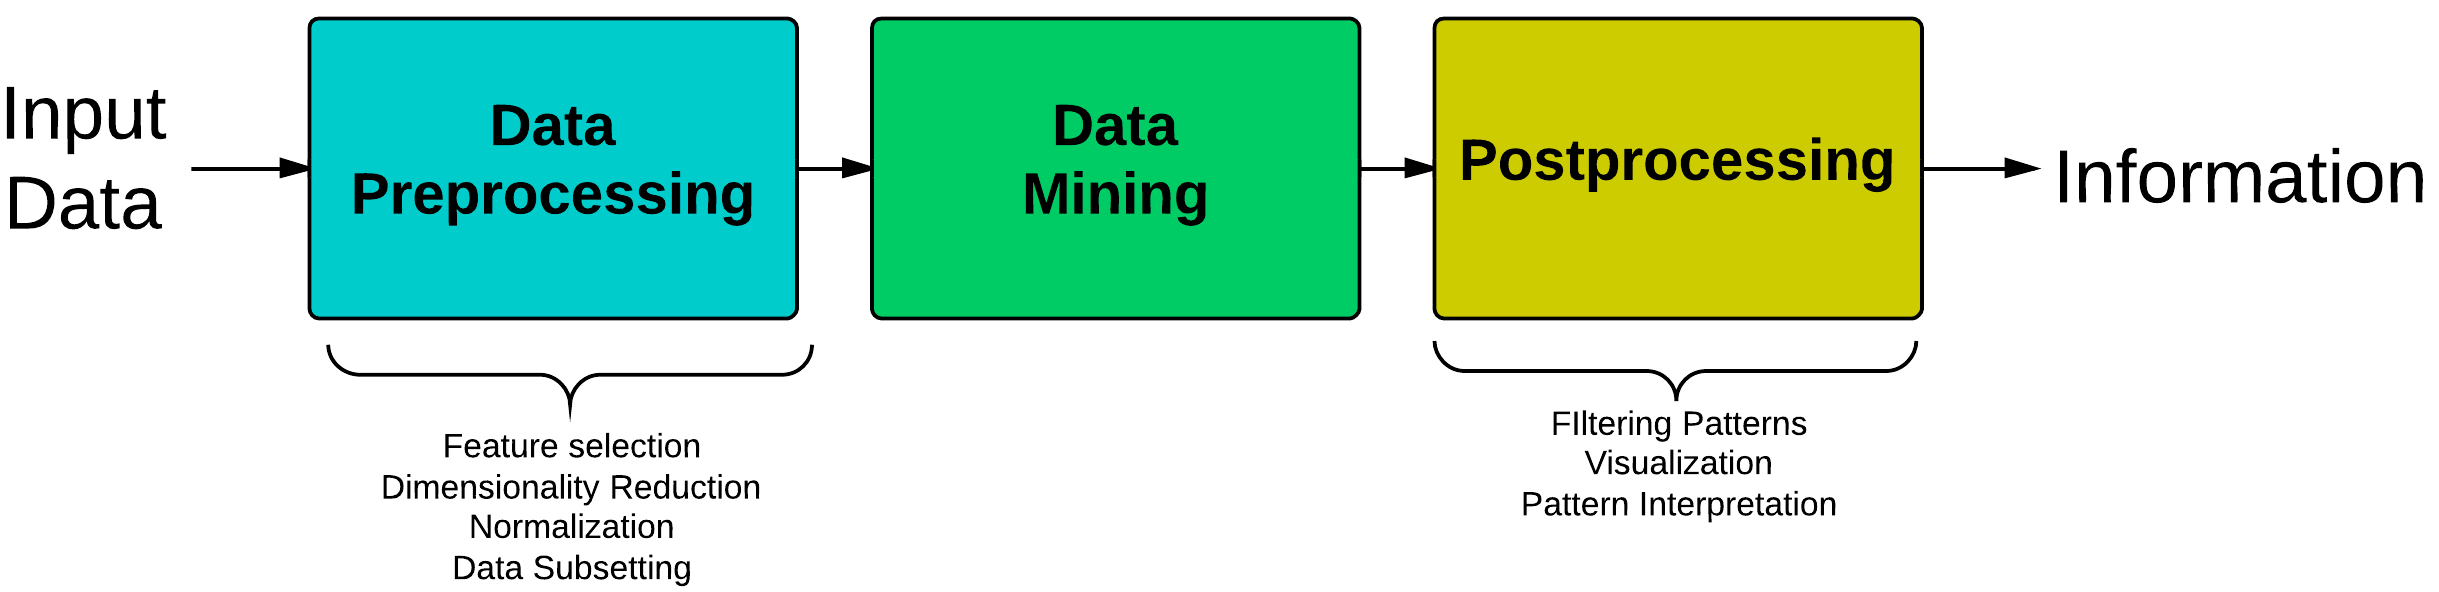
\includegraphics[width=\textwidth]{pics/KDD.png}
		\end{figure}

	\clearpage
	%http://dataminingwarehousing.blogspot.no/2008/10/data-mining-steps-of-data-mining.html
	The process of knowledge discovery in databases (blogpost)
		
	\begin{enumerate}
		\item {\bf Data Integration:} First of all the data are collected and integrated from all the 
		different sources.
		\item {\bf Data Selection:} We may not all the data we have collected in the first step. So in this 
		step we select only those data which we think useful for data mining.
		\item {\bf Data Cleaning:} The data we have collected are not clean and may contain errors, missing values,
		noisy or inconsistent data. So we need to apply different techniques to get rid of such anomalies.
		\item {\bf Data Transformation:} The data even after cleaning are not ready for mining as we need to 
		transform them into forms appropriate for mining. The techniques used to accomplish this are smoothing,
		aggregation, normalization etc.
		\item {\bf Data Mining:} Now we are ready to apply data mining techniques on the data to discover the 
		interesting patterns. Techniques like clustering and association analysis are among the many different
		techniques used for data mining.
		\item {\bf Pattern Evaluation and Knowledge Presentation:} This step involves visualization, 
		transformation, removing redundant patterns etc from the patterns we generated.
		\item {\bf Decisions / Use of Discovered Knowledge:} This step helps user to make use of the knowledge acquired to take better decisions.
	\end{enumerate}

		\begin{figure}[H]
			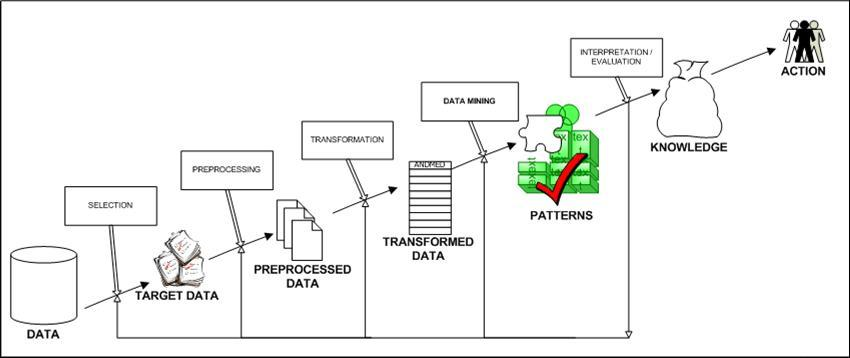
\includegraphics[width=\textwidth]{pics/datamining.jpg}
		\end{figure}

\clearpage
\section{Motivating Challenges}

	\begin{itemize}
		\item {\bf Scalability:} the massive explosion of saved data are becoming common. If data mining 
		algorithms are to handle these massive data sets, then they must be scalable.
		\item {\bf High Dimensionality:} It is now common to encounter data sets with hundres or thousands 
		of attributes instead of the handful common a few decades ago. This affects the algorithms used 
		because of the computational complexity increase rapidly as the dimensionality (thw number of 
		features) increases.
		\item {\bf Heterogeneous and Complex Data:} Data is often in a different format and contain different
		information. This makes it difficult to preprocess and analyse the data. The data that is collected is
		often very complex in terms of location, format, content and size. 
		\item {\bf Data Ownership and Distribution:} sometimes, the data needed for an analysis is not 
		stored in one location or owned by one organization. Instead, the data is geographically distributed 
		among resources belonging to multiple entities. This requires the development of distributed
		data mining techniques. 
		\item {\bf Non-traditional Analysis:} 
	\end{itemize}

\clearpage
\section{Data Mining Tasks}
	
	{\bf Data mining tasks are generally divided into:}

	\begin{itemize}
		\item {\bf Descriptive tasks:} The objective of these tasks is to predict 
		the value of a particular attribute based on the values of other attributes. 
		The attribute to be predicted is commonly known as the {\bf target} or 
		{\bf dependent variable}, while the attributes used for making the prediction are 
		known as the {\bf explanatoy} or {\bf independent variables}. 
		{\bf Examples: }{\color{blue} Classification, regression, anomalies detection} 
		\item {\bf Predictive tasks:} Here, the objective is to derive patterns 
		(correlations, trends, custers, trajectories, and anomalies) that summarize the undelying relationships in data. Descriptive data mining tasks are often exploratory in nature 
		and frequently require postprocessing tecniques to validate and explain the results. 
		{\bf Examples:} {\color{blue}Clustering, association rules and sequence patterns.}
	\end{itemize}

	{\bf The core data mining tasks:}
	\begin{itemize}
		\item {\bf Cluster Analysis:} seeks to find groups of closely related observations
		so that observations that belong to the same cluster are more similar to each other
		than observarions that belong to other clusters.
		\item {\bf Predictive Modeling:} refers to the task of building a model for the 
		target variable as a function of the explanatory variables. There are two types of 
		predictive modeling tasks: {\bf classification}, which is used for descrete target 
		variables, and {\bf regression}, which is used for continuous target variables. 
		\item {\bf Anomaly detection:} is the task of identifying observations whose 
		characteristics are significantly different from the rest of the data. Such observations
		are known as {\bf anomalies} or {\bf outliners}.
		\item {\bf Association Analysis:} is used to discover patterns that describe strongly
		associated features in the data. The discovered patterns are typically represented in the 
		form of implication rules or feature subsets. 
	\end{itemize}

	\begin{figure}[H]
		\centering
		\subfigure{
			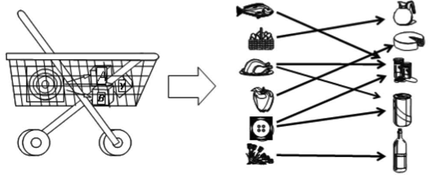
\includegraphics[scale=0.5]{pics/association.png}
		}
		\subfigure{
			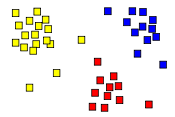
\includegraphics[scale=0.6]{pics/cluster.png}
		}
		\subfigure{
			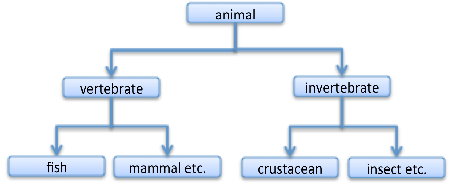
\includegraphics[scale=0.5]{pics/classification.png}
		}
		\subfigure{
			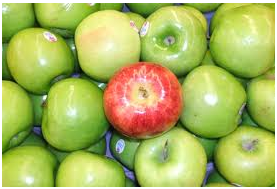
\includegraphics[scale=0.6]{pics/anomlay.png}
		}
		\caption{Association analysis, cluster analysis, classification (predictive) 
		and anomaly detction}
	\end{figure}

\section{The Origins of Data Mining}

	Data mining as a confluence of many disciplines:

	\begin{figure}[H]
		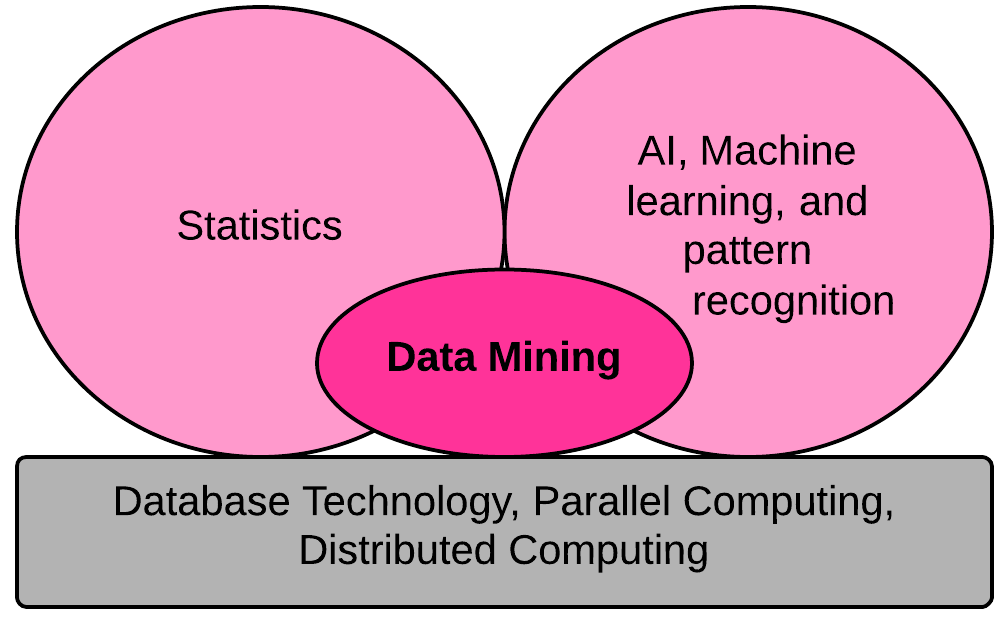
\includegraphics[scale=0.3]{pics/disciplinesDataMining.png}
	\end{figure}



	


	\clearpage
	\chapter{Data}
\clearpage

\section{Types of Data}
	
	\begin{itemize}
		\item {\bf Data set: } collection of data objects.
		\item {\bf Data Objets: } often called record, point, vector, pattern, event, case,
		sample, observation or entity. Data objects are described by a number of attributes
		that capture the basic characteristics of an object.
		\item {\bf Attributes: } other names used are variable, characteristic, field, feature, 
		or dimension. An attribute is a property or characteristic of an object that may
		vary, either from one object to another or from time to another.
		\item {\bf Measurement scale: } is a rule (function) that associates a numerical or
		symbolic value with an attribute of an object. It is important to understand the 
		mesurement. An attribute can be an integer like ID and age. They are both integers, 
		but it does not mean that we can calculate the average ID numer like we can calculate
		the average age. Note that is common to refer to the type of an attribute as the
		{\bf type of a measurement scale}.
	\end{itemize}

	\subsection*{Types of Attributes}
	{\bf Categorical types (Qualitative):} Nominal and Ordinal

	{\bf Numeric types (Quantitative):} Interval and Ratio

		\begin{figure}[H]
			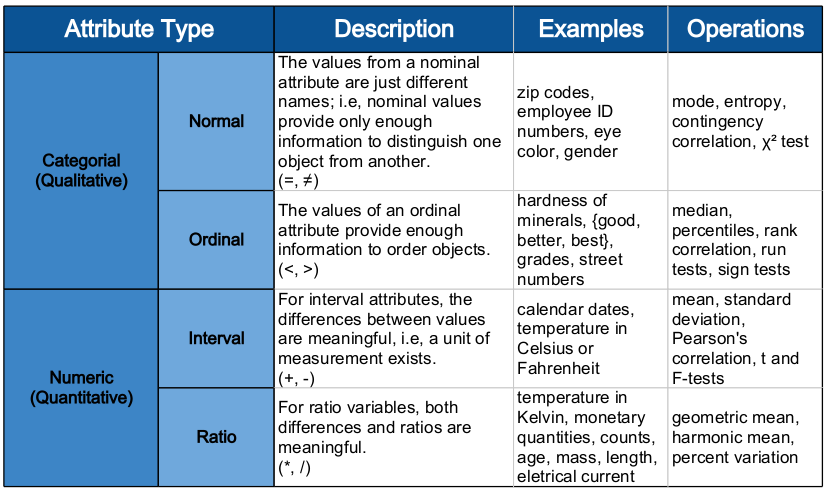
\includegraphics[width=\textwidth]{pics/typeOfAttributes.png}
		\end{figure}

	\clearpage
	\subsection*{Transformations}

		The types of attributes can be described in terms of transformations that
		do not change the meaning of an attribute. 

		\begin{figure}[H]
			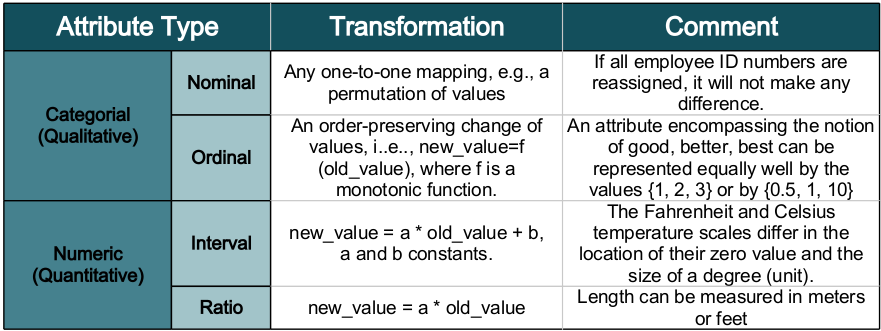
\includegraphics[width=\textwidth]{pics/transformations.png}
		\end{figure}

	\subsection*{Attributes by the Number of Values}

	An independent way of distinguishing between attributes is by the number of values
	they can take.

	\begin{itemize}
		\item {\bf Discrete:} A discrete attribute has a finite or countably infinite
		set of values. {\bf Binary attributes} are a special case of discrete attributes. 
		\item {\bf Continnuous:} A continuous attribute is one whose values are real numbers.
		\item {\bf Asymmetric:} For asymmetric attributes, only presence - a non-zero attribute
		value - is regarded as important. Binary attributes where only non-zero values are 
		important are called asymmetric binary attibutes. We can take a look at a list of all 
		courses at NTNU. If we look at a particular student, the chance for a particular student
		have taken a exam in a course from the whole list is quite small. It is only the non-zero
		values that are important. 
	\end{itemize}

	\clearpage
	\section{Type of Data Sets}

		\subsection*{General Characteristics of Data Sets}
			\begin{itemize}
				\item {\bf Dimensionality:} is the number of attributes that the object in the 
				class set possess.
				\item {\bf Sparsity:} for some data sets, such as asymmetric features, most
				attributes of an object have values of 0. In practical terms, sparsity is an advantage
				because usually only the non-zero values need to be stored an manipulated. 
				\item {\bf Resolution:} it is frequently possible to obtain data at different levels of
				resolution, and often the properties of the data are different at different resoultions.
				F.eks the surface of the Earth seems very uneven at a resolution of a few meters, but is *
				relatively smooth at a resolution of ten kilometers. The patterns in the data also depend
				on the level of resolution. Too fine will might hide the pattern or be buried in noise if
				to uneven. 
			\end{itemize}


		\clearpage
		\subsection*{Record Data}
		Much data mining work assumes that the data set is a collection of records (data objects), each of which consists of a fixed set of data fields (attributes).
			\begin{itemize}
				\item {\bf Transactions or Market Basket Data:} transaction data is a sepecial type of record
				data, where each record (transaction) involves a set of items. Transaction data is a collection
				of sets of items. 
				\item {\bf The Data Matrix:} if the data objects in a collection of data all have the
				same fixed set of numeric attributes, then the data objects can be thought of as points
				(vectors) in a multidimensional space, where each dimension represents a distinct attribute
				describing the object. 
				\item {\bf The Sparse Data Matrix:} A sparse data matrix is a special case of a data matrix in
				which the attributes are some of the same type and are symmetric; i.e, only non-zero values
				are important. {\bf Document-term matrix } is one type. 
			\end{itemize}

		\begin{figure}[H]
			\centering
			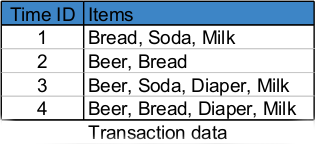
\includegraphics[scale=0.5]{pics/transactionData.png}
		\end{figure}

		\begin{figure}[H]
			\centering
			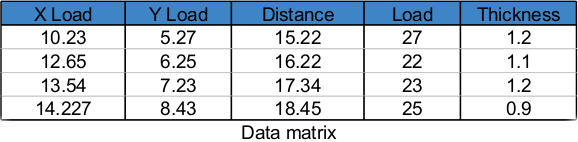
\includegraphics[scale=0.5]{pics/dataMatrix.png}
		\end{figure}

		\begin{figure}[H]
			\centering
			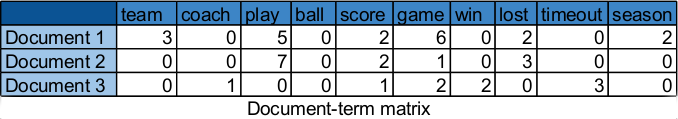
\includegraphics[scale=0.5]{pics/DocumentTermMatrix.png}
		\end{figure}

		\subsection*{Graph-Based Data}
			\begin{itemize}
				\item {\bf Data with Relationships among Objects:} the relationships among objects frequently convey important information. In such cases, the data is often represented as a graph. In 
				particular, the data objects are mapped to nodes of the graph, while the relationships among
				objects are captured by the links between objects and link propeties. 
				\item {\bf Data with Objects Thar Are Graphs:} if objects have structure, that is, the objects
				contain subobjects that have relationships, then such objects are frequently represented as graphs.
			\end{itemize}

		\clearpage
		\subsection*{Ordered Data}
		For some types of data, the attributes have relationships that involve order in time or space. 
			\begin{itemize}
				\item {\bf Sequential Data (temporal data):} can be thought of as an extension of record data, 
				where each record ha a time associated with it. 
				\item {\bf Sequence Data:} consists of a data set that is a sequence of individual entities, 
				such as a sequence of words or letters. 
				\item {\bf Time Series Data:} is a special type of sequential data in which each record is a
				time series, i.e, a series of measurements taken over time. 
				\item {\bf Spatial Data:} some objects have spatial attributes, such as positions or areas, as
				well as other type of attributes. 
			\end{itemize}

		\begin{figure}[H]
			\centering
			\subfigure{
				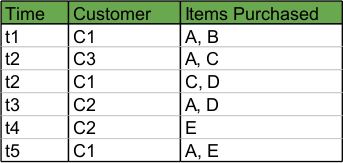
\includegraphics[scale=0.5]{pics/transactionData1.png}
			}
			\subfigure{
				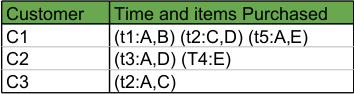
\includegraphics[scale=0.5]{pics/transactionData2.png}
			}
			\caption{Sequential transaction data}
		\end{figure}

		\begin{figure}[H]
			\centering
			\subfigure{
				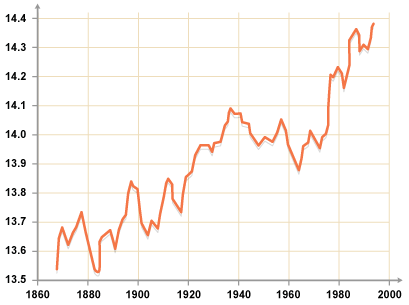
\includegraphics[scale=0.4]{pics/timeSeries.png}
			}
			\subfigure{
				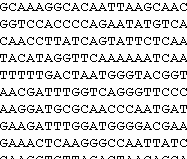
\includegraphics[scale=0.7]{pics/GenomicSequence.png}
			}
			\caption{Temperature time series and Genomic sequence data}
		\end{figure}

		\begin{figure}[H]
			\centering
			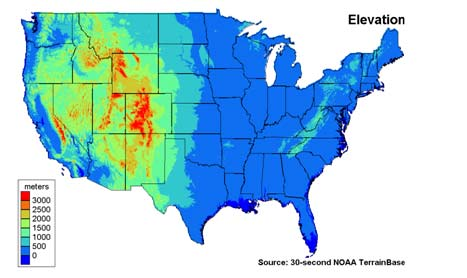
\includegraphics[scale=0.5]{pics/spatialTemp.jpg}
			\caption{Spatial temperature data}
		\end{figure}


\section{Data Quality}
	
	{\bf Data mining focuses on:}
	\begin{enumerate}
		\item The detection and correction of data quality problems (data cleaning).
		\item The use of algorithms that can tolarate poor data quality
	\end{enumerate}

	{\bf Measurement error:}
		\begin{itemize}
			\item {\bf Noise}
			\item {\bf Artifacts:} data errors may be the result of a more deterministic
			phenomenon, such as a streak in the same place on a set of photographs.
			\item {\bf Bias:} a systematic variation of measurements from the quanity
			being measured. 
			\item {\bf Precision:} the closeness of repeated measurements (of the
			same quantity) to one another.
			\item {\bf Accuracy:} the closeness of measurements to the true value
			of quantity being measured.
		\end{itemize}

	{\bf Data collection problems:}
		\begin{itemize}
			\item {\bf Outliners:} Outliners are either (1) data objects that, in some
			sense, have characteristics that are different from most of the other data
			objects in the data set, or (2) values of an attribute that are unusual with
			respect to the typical values for that attribute. It is important to distinguish
			between the notions of noise and outliners. Outliners can be legitimate data
			objects or values, unlike noise, outliners may sometimes be of interest. 
			\item {\bf Missing values:} it is not unusual for an object to be missing one 
			or more attribute values. Here are some strategies for dealing with missing values:
				\begin{itemize}
					\item Eliminate data object or attributes
					\item Estimate missing values
					\item Ingnore the missing value during analysis
				\end{itemize}
			\item {\bf Inconsistent values:} it often detected inconsistent data with manual
			typing or handwriting. It is important to correct the data as soon as possible.
			\item {\bf Duplicate data:} Often detected when there exists two objects that 
			acyually represent a single object. 
		\end{itemize}

	{\bf Issues Related to Applications}
		\begin{itemize}
			\item {\bf Timeliness:} some data starts to age as soon as it had been 
			collected. If the data is out of date, then so are the models and patterns
			that are based on it. 
			\item {\bf Relevance:} the available data must contain the information necessary
			for the application. Lack of information could give a wrong impression or patterns.
			\item {\bf Knowledge about the data:} important characteristics like precision of the
			data, the type of features (nominal, ordinal, interval, ratio), the scale of 
			measurement (e.g., meters or feet for length), and the origin of the data.
		\end{itemize}

		\vspace{1cm}

		{\LARGE "...data is of high quality if it is suitable for its intended use"}



\section{Data Preprocessing}
	
	\subsection*{Aggregation}
		\begin{itemize}
			\item Sometimes {\bf "less is more"} and this is the case with aggregation, 
			the combining of two or more objects into a single object. 
			\item {\bf Motivations for aggregation:}
				\begin{enumerate}
					\item The smaller the data sets resulting from data reduction
					require {\bf less memory and processing time}.
					\item aggregation may permit the use of {\bf expensive data mining 
					algorithms}
					\item Aggregation can act as a change of scope or scale by providing a
					high-level view of the data instead of a low-level view. 
					\item The behaviour of groups of objects or attributes is often {\bf more
					stable} than that of individual objects or attributes. 
				\end{enumerate}
			\item A {\bf disadvantage} of aggregation is the potential loss of interesting details. 
			An a store example aggregating over monthhs loses information about which day of the
			week has the highest sales. 
		\end{itemize}

	\subsection*{Sampling}
		\begin{itemize}
			\item {\bf Sampling} is a commonly used approach for selecting a subset of the data 
			objects to be analyzed. To analyze a full data set if often too expensive or 
			time consuming. 
			\item The key principle for effective sampling is the following: Using a sample
			will work almost as well as using the entire data set if the sample is 
			representative.
			\item {\bf A sample is representative if} it has approximately the same property 
			(of interest) as the original set of data. If the mean (average) of the data
			objects is the property of interest, then a sample is representative if it has
			a mean that is close to that of the original data. 
			\item {\bf Sampling approaches:}
				\begin{itemize}
					\item {\bf Simple random sampling: } for this type of sampling there is 
					an equal probability of selecting any particular item. There are two 
					variations on random sampling
						\begin{enumerate}
							\item {\bf Sampling without replacement:} as each item is selected, it is
							removed from the set of all objects that together constitute the
							population. 
							\item {\bf Sampling with replacement:} objects are not removed from 
							the population as they are selected for the sample. 
						\end{enumerate}
					{\bf Pros and cons with random sampling:}  
					(1) Sampling with replacement are is simpler to analyze since the probability 
					of selecting any object remains constant during the sampling process. 
					(2) When the population consists of different types of objects, with widely
					different numbers of objects, simple random sampling can fail to adequately
					represent those types of objects that are less frequent. This can cause
					problems when the analysis require proper representation of all object types.
					\item {\bf Stratified sampling:} starts with prespecified groups of objects.
						\begin{enumerate}
							\item In the simplest version, equal numbers of objects are drawn from 
							each group even though the groups are of different sizes. 
							\item In an other variation, the number of objects drawn from each group 
							is proportional to the size of that group. 
						\end{enumerate} 
					\item {\bf Adaptive and progressive sampling:} The proper sampling size
					can sometimes be difficult to determine. These approaches starts with a 
					small sample, and then increase the sample size until a sample of sufficient
					size has been obtained. While this technique eliminates the need to determine
					the correct sample size initially, it requires that there be a way to evaluate
					the sample to judge if it is large enough.
				\end{itemize}			
		\end{itemize}

	\subsection*{Dimensionality reduction}
		\begin{itemize}
			\item Example of data sets with a high dimentionality is a object with many
			attributes like a document object where each word in the document is an 
			attribute. 
			\item There is a varity of benefits to dimensionality reduction. A key benefit 
			is that many data mining algoithms work better if the dimensionality - 
			the number of attributes in the data - is lower. This is partly because 
			dimensionality reduction can eliminate irrelevant features and reduce noise and
			partly because of the curse of dimensionality.
			\item Another benefit is that a reduction of dimensionality can lead to a more
			understandable model because the model may involve fewer attributes.
			\item Dimensionality reduction may allow the data to be more easily visualzed.
			\item The amount of time and memory required by the data mining algorithm is reduced 
			with a reduction in dimensionality. 
			\item The term dimensionality reduction is often reserved for those techniques
			that reduce the dimensionality of a data set by creating new attributes that
			are a combination of the old attributes. 
			\item {\bf The curse of dimensionality:} the curse of dimensionality refers
			to the phenomen that many types of data analysis become significantly harder
			as the dimensionality of the data increases. 
			\item {\bf Linear alegebra techniques for dimensionality reduction:} some
			of the most common approaches for dimensionality reduction, poarticulary for
			continous data, use techniques from linear algebra to project the data from a 
			high-dimensional space into a lower-dimensional space. 
				\begin{itemize}
					\item {\bf Principal Components Analysis (PCA):} is a linear algebra technique 
					for continuous attributes that finds new attributes (principal components)
					that (1) are linear combinations of the original attributes, 
					(2) are orthogonal to each other, and (3) capture the maximum amount of 
					variation in the data. 
					\item {\bf Singular value decomposition (SVD): } is a linear algebra
					technique that is related to PCA and is also commonly used for
					dimensionality reduction.
				\end{itemize}
		\end{itemize}

	\clearpage
	\subsection*{Feature subset selection}
		\begin{itemize}
			\item A way to reduce the dimensionality is to use only a subset of the 
			features.
			\item {\bf Redundant and irrelevant features:} redundant features duplicate much 
			or all of the information contained in one or more other attributes. Irrelevant
			features contain almost no useful information for the data mining task at hand
			(feks ID number will not be relevant if we want to predict students grade).
			\item {\bf Approaches for feature selection:}
				\begin{itemize}
					\item {\bf Embedded approaches:} feature selection occurs naturally as
					a part of the data mining algorithm.
					\item {\bf Filter approaches:} features are selected before the data
					mining algorithm is run, using some approach that is independent of the
					data mining task. 
					\item {\bf Wrapper approaches:} these methods use the target data mining
					algorithm as a black box to find the best subset of attributes, in a way
					similar to that of the ideal algorithm described above, but typically 
					without enumerating all possible subsets. 
				\end{itemize}
			\item{\bf An architecture for feature subset selection:} 
			a measure for evaluating a subset, a search strategy that controls the generation 
			of a new subset of features, a stopping criterion, and a validation procedure.
				\begin{figure}[H]
					\centering
					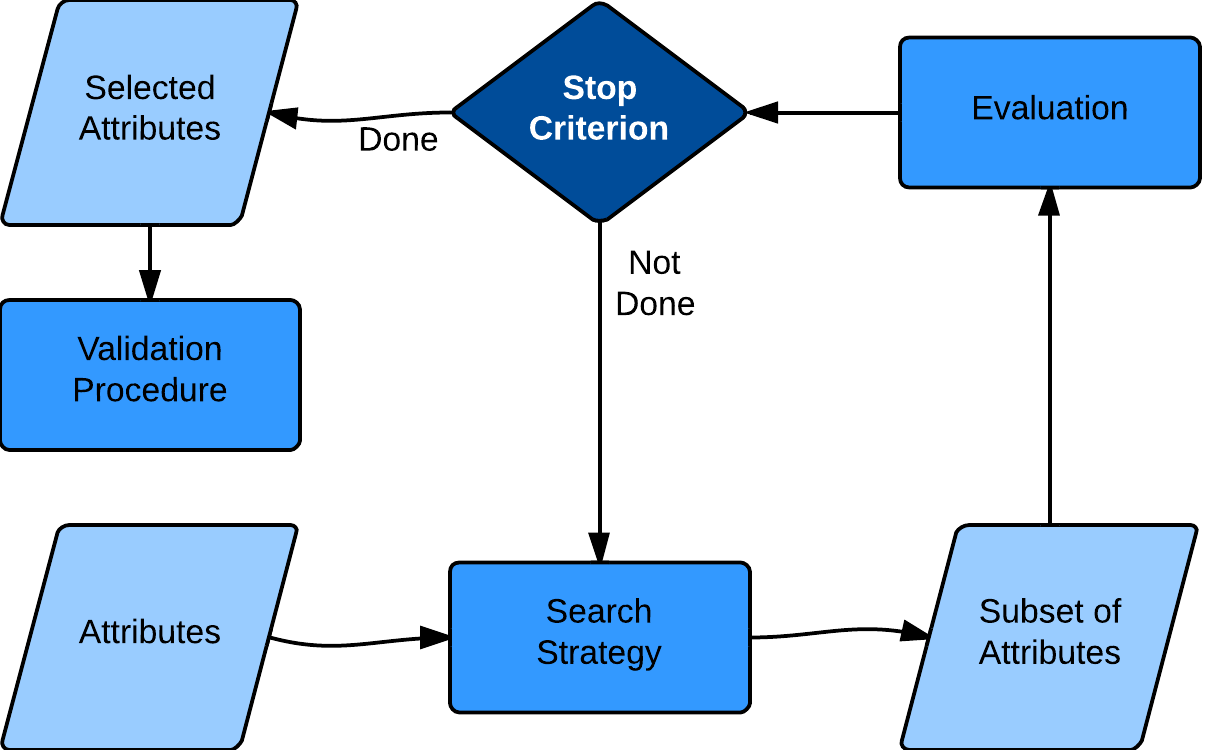
\includegraphics[scale=0.2]{pics/featureSelection.png}
				\end{figure} 
			\item{\bf Feature Wighting:} is an alternative to keeping or eliminate features.
			More important features are assigned a higher weight, while less important
			features are given a lower weight. 
		\end{itemize}

	\subsection*{Feature creation}
		\begin{itemize}
			\item It is frequently possible to create, from the original attributes, a new set
			of attributes that captures the important information in a data set much more
			effectively. 
			\item {\bf Feature extraction:} the creation of a new set of features from the 
			original raw data. 
			\item {\bf Mapping the data to a new space:} 
			\item {\bf Feature Construction: } sometimes the features in the original data sets have
			the necssary information, but is not in a form suitable for the data mining algorithm.
			In this situation, one or more new features constructed out of the original features can
			can be more useful than the original features. 
		\end{itemize}

	\subsection*{Discretization and binarization}
		\begin{itemize}
			\item Some data mining algorithms, especially certain classification algorithms, 
			require that the data be in the form of categorical attributes. 
			\item {\bf Discretization:} It is often necessary to transform a continuous attribute into a categorical attribute.
			\item {\bf Binarizaation:} both continuous and discrete attributes may need to be 
			transformed into one or more binary attributes.
			\item If a categorical attribute has a large numer of values (categories), or some
			values occur infrequently, then it may be beneficial for certain data mining tasks
			to reduce the number of categories by combining some of the values. 
		\end{itemize}

	\subsection*{Variable transformation}
		\begin{itemize}
			\item A {\bf variable transformation} refers to a transformation that is applied to
			all the values of a variable. 
			\item{\bf Types of variable transformations:}
				\begin{itemize}
					\item{\bf Simple functions:} for this type of variable transformation, a 
					simple mathematical function is applied to each value individually. 
					\item{\bf Normalization and standardization:} the goal of standardization 
					or normalization is to make an entire set of values have a particular 
					property. 
				\end{itemize}
		\end{itemize}

\section{Measures of Similarity and Dissimilarity}





	\clearpage
	\chapter{Exploring Data}
	\clearpage
	\chapter{Classification: Basic Concepts, Decision Trees, and Model Evaluation}

	{\bf Classification} is the task of assigning objects to one of several
	predefined categories, or in other words, classification is the task
	of mapping an input attribute set x into its class label y.

	\begin{figure}[H]
		\centering
		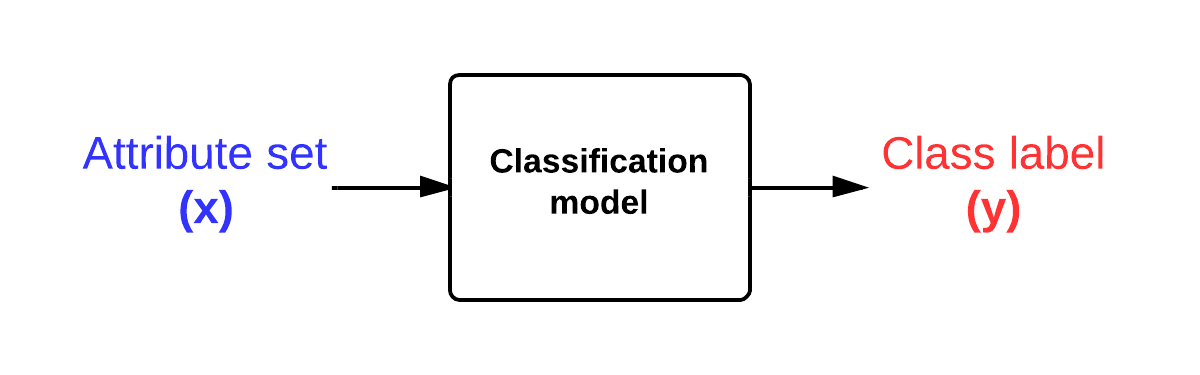
\includegraphics[width=\textwidth]{pics/classification2.png}
	\end{figure}

	\clearpage

	\section{Preliminary}

		The input data for a classification task is a collection of records.
		Each record, also known as an instance or example, is characterized
		by a tuple ({\bf x}, y), where {\bf x} is the attribute and set and
		y is a special attribute called a classification class (class label).

		The attribute set can be descrete and continuous, but the class label
		is always a descrete value. 

		{\bf Definition classification:} classification is the task of
		learning a taget function f that maps each attribute set {\bf x}
		to one of the predifined class labels y.

		The target function is also known as a classification model.
		A classification model is useful for the following purposes:
			\begin{itemize}
				\item {\bf Descriptive Modeling:} can use the class label that
				explains what features defines a object (class label $\rightarrow$ features)				
				\item {\bf Predictive Modeling:} a classification model can be
				used to predict the class label of unknown records. (features $\rightarrow$ class label)
			\end{itemize}

	\section{General Approach to Solving a Classification Problem}

		{\bf Learning algorithm:} identifies a model that best fits the relationships
		between the attribute set and class label of input data. Examples of learning 
		algorithms are: decision tree classifiers, rule-based classifiers, neural networks, 
		support vector machines, and naive Bayes classifiers. 

		{\bf Traing set:} consists of records whose class labels are known must be provided.
		The training set is used to build a classification model, which is subsequently aapplied
		to the test set.

		{\bf Test set:} consists of records with unknown class labels.

		\begin{figure}[H]
			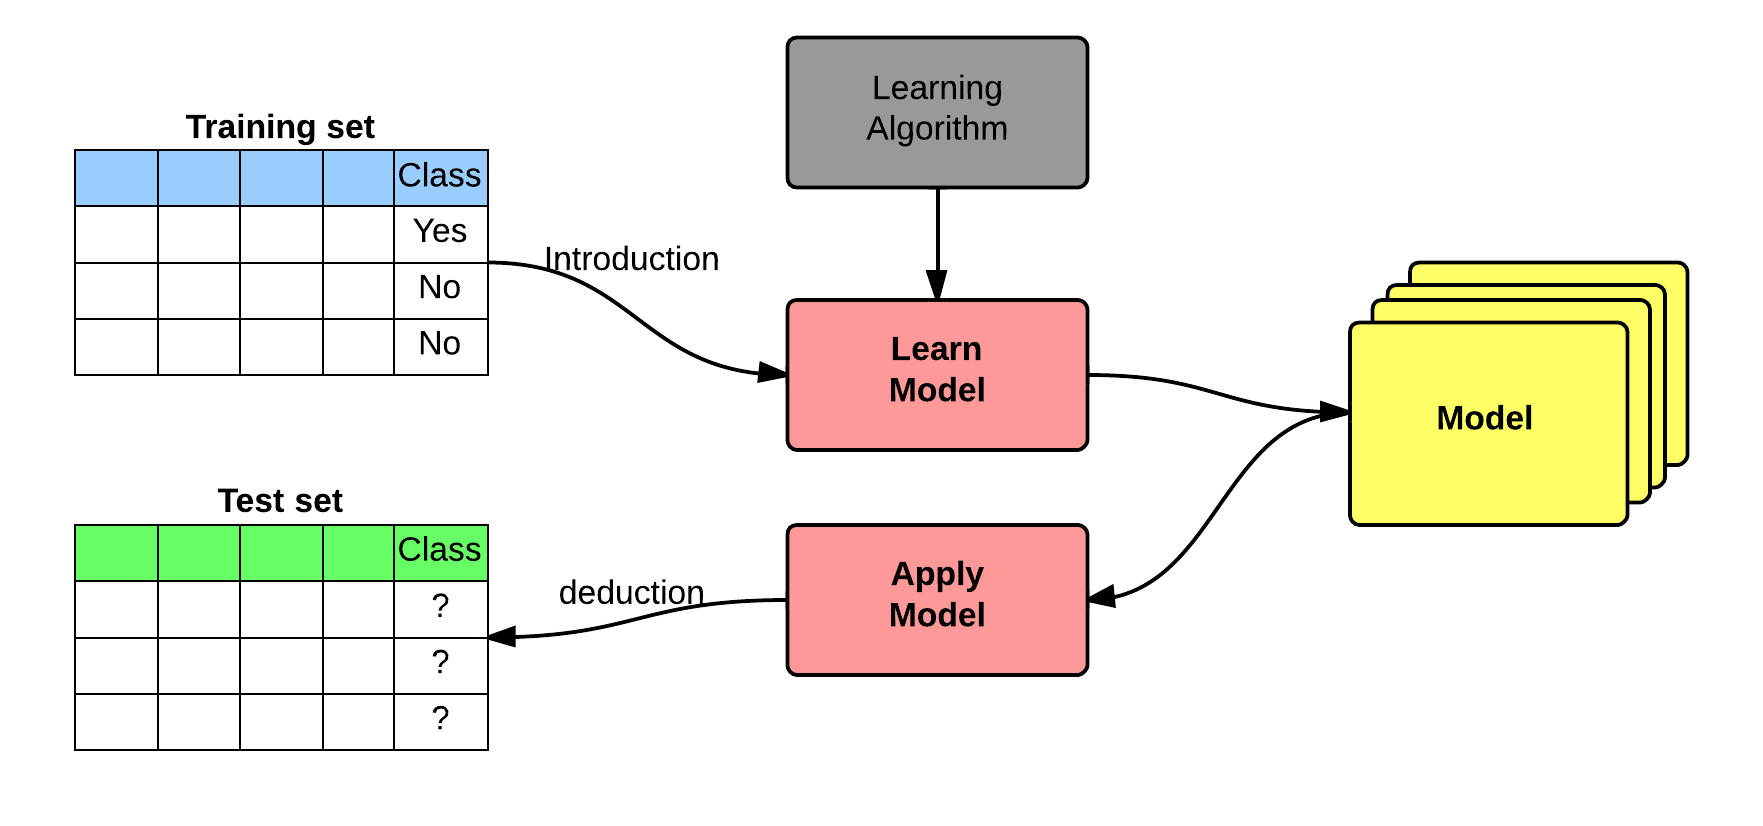
\includegraphics[width=\textwidth]{pics/classification3.png}
		\end{figure}

		{\bf Confusion matrix:} evaluation of classification model is based on the coounts of
		test records correctly and incorrectly predicted by the model. The results are known
		as a confusion matrix. The perfromance can be calculated with accuracy or error rate
		which uses the numbers from the confusion matrix. 

		\begin{table}[H]
		\centering
			\begin{tabular}{| l | l | l | l |}
				\hline
				\multicolumn{2}{| l |}{\multirow{2}{*}{ }} & \multicolumn{2}{| l |}{Predicted class} \\ \cline{3-4} 
				 & & Class = 1 & Class = 0 \\ \hline
				\multirow{2}{*}{Actual class} & Class = 1 & $f_{11}$ & $f_{10}$ \\ \cline{2-4}
					& Class = 0 & $f_{01}$ & $f_{00}$ \\ \hline

			\end{tabular}
			\caption{Confusion matrix for a 2-class problem.}
		\end{table}

		\begin{equation}
			Accuracy = \frac{Number of correct predictions}{Total number of predictions} =
			\frac{f_{11} + f_{00}}{f_{11} + f_{10} + f_{01} + f_{00}}
		\end{equation}
		\begin{equation}
			Error rate = \frac{Number of wrong predictions}{Total number of predictions} =
			\frac{f_{10} + f_{01}}{f_{11} + f_{10} + f_{01} + f_{00}}
		\end{equation}

	\section{Decision Tree}

		We can solve a classification problem by asking a series of carefully
		crafted questions about the attributes of the test record. 
		Each time we recieve an answer, a follow-up question is asked until
		we reach a conclusion about the class label of the record. The series
		of question and their possible answers can be organaized in the form of
		a decision tree, which is a hierarchical structure consisting of nodes
		and directed edges.

		\begin{itemize}
			\item {\bf A root node} has no incoming edges and zero or more outgoing edges
			\item {\bf Internal nodes}, each of which has exactly one incoming edge and 
			two or more outgoing edges. An internal node is a new question.  
			\item{\bf Leaf/terminal nodes} , each of which has exactly one incoming edge
			and no icoming edges. Is a class label. If a leaf node is reached, you got the
			conclusion. 
		\end{itemize}

		\begin{figure}[H]
			\centering
			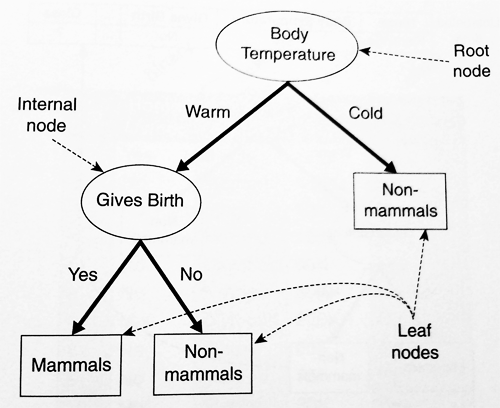
\includegraphics[scale=0.4]{pics/decision.png}
		\end{figure}

		There is many ways to construct a decision tree. There is many known algorithms to
		do this: Hunt's algorithm, ID3, C4.5 and CART. 

\clearpage
		{\bf Hunt's algorithm:} let $D_{t}$ be the set of training records that are 
		associated with node t and y = {$y_{1}, y_{2}, ...., y_{c}$} be the class labels. 
		This is a recursive definition of Hunt's algorithm:
		\begin{enumerate}
			\item If all the records in $D_{t}$ belongs to the same class $y_{t}$, then
			t is a leaf node labeled as $y_{t}$
			\item If $D_{t}$ contains records that belong to more than one class, an
			attribute test condition is selected to partiotion the records into smaller
			subsets. A child node is created for each outcome of the test condition and 
			the records in $D_{t}$ are distributed to the childdren based on the outcomes. 
			The algorithm is then recursively applied to each child node. 
		\end{enumerate} 

		Hunt's algorithm will work if every combination of attribute values is present
		in the training data and each combination has a unique class label. 
		These assuptions are too stringent for use in most practical situations. 
		Additional conditions are needed to handle the following cases:

		\begin{enumerate}
			\item {\bf Empty child nodes:} in this case the node is declared a leaf
			node with the same class label as the majority class of training records
			associated with its parent node. 
			\item{\bf Identical attribute values:} if all the records associated with
			$D_{t}$ have identical attribute values (expect for the class label), then
			it is not possible to split these records any further. In this case, the node is
			declared a leaf node with the same class label as the majority class of 
			training records associated with this node.
		\end{enumerate}

		{\bf Design issues of decision trees}
			\begin{itemize}
				\item How should the training records be split?
				\item How should the splitting procedure stop?
			\end{itemize}

	\subsection{Methods for Expressing Attribute Test Conditions}

		{\bf Binary Attributes:} Have only 2 potential outcomes.

		{\bf Nominal Attributes:} Can have many values, so you can either have
		a multiway split (split for each value) or have a binary split by grouping
		the values. 

		{\bf Ordinal Attributes:} ordnal values can be handeled in the same way as
		nominal attributes, except that the values have an order. It does not make
		sense to combine the values "small, large" and "medium, extra large". To do
		a binary split, you would have to group feks "small, medium" and "large, extra large".

		{\bf Continuous Attributes:} here you can use a test condition expressed as a
		comparison with binary outcomes (A $<$ v or A$>$v), or a range query with outcomes 
		with multiple values. 

	\clearpage
	\subsection{Measures for Selecting the Best Split}
		$p(i|t)$ is the fraction of records belonging  to class i at a given node t.		
		c is the number of classes.
		Here are three different impurity measures: 
		\begin{equation}
			Entropy(t) = -\sum_{i=0}^{c-1} p(i|t)log_{2}p(i|t)
		\end{equation}

		\begin{equation}
			Gini(t) = 1 - \sum_{i=0}^{c-1}[p(i|t)]^{2}
		\end{equation}
		\begin{equation}
			Classification error(t) = 1 - max_{i}[p(i|t)]
		\end{equation}

		\begin{table}[H]
		\centering
		\begin{tabular}{ l l }
			 \hline
			\begin{tabular}{|l|l|}
				\hline
				\rowcolor{gray}
				Node $N_{1}$ & Count \\ \hline
				Class=0 & 0 \\ \hline
				Class=1 & 6 \\ \hline
			\end{tabular}
		& 
			\begin{tabular}{l}
				Gini = 1 - $(0/6)^{2}$ - $(6/6)^{2}$ = 0 \\
				Entropy = -(0/6)$log_{2}$(0/6) - (6/6)$log_{2}$(6/6) = 0 \\ 
				Error = 1-$max[(0/6), (6/6)] = 0$ \\
			\end{tabular}

 		\\ \hline

			\begin{tabular}{|l|l|}
				\hline
				\rowcolor{gray}
				Node $N_{2}$ & Count \\ \hline
				Class=0 & 1 \\ \hline
				Class=1 & 5 \\ \hline
			\end{tabular}
		&
			\begin{tabular}{l}
				Gini = 1 - $(1/6)^{2}$ - $(5/6)^{2}$ = 0.278  \\
				Entropy = -(1/6)$log_{2}$(1/6) - (5/6)$log_{2}$(5/6) = 0.650  \\
				Error = 1-$max[(1/6), (6/6)] = 0.167$
			\end{tabular}	
		\\ \hline

			\begin{tabular}{|l|l|}
				\hline
				\rowcolor{gray}
				Node $N_{3}$ & Count \\ \hline
				Class=0 & 3 \\ \hline
				Class=1 & 3 \\ \hline
			\end{tabular}
		& 
			\begin{tabular}{l}
				Gini = 1 - $(3/6)^{2}$ - $(3/6)^{2}$ = 0.5 \\
				Entropy = -(3/6)$log_{2}$(3/6) - (3/6)$log_{2}$(3/6) = 1 \\
				Error = 1-$max[(3/6), (3/6)] = 0.5$ 
			\end{tabular}
		\\ \hline
		\end{tabular}
		\end{table}

		To determine how well a test condition performs, we need to compare the 
		degree of impurity of the parent node (before splitting) with the degree
		of impurity of the child nodes (after splitting). The larger the difference,
		the better the test condition. The gain $\Delta$, is a criterion that can 
		be used to determine the goodness of a split. 

			\begin{equation}
				\Delta = I(parent) - \sum_{j=1}^{k} \frac{N(v_{j})}{N}I(v_{j})
			\end{equation}

		I(.) is the impurity measure of a given node, N is the total number
		of records at the parent node, k is the number of attribute values, 
		and N($v_{j}$) is the number of records associated with the child node, $v_{j}$.
		When entropy is used as the impurity measure in equation 4.6, the difference
		in entropy is known as the {\bf information gain}, $\Delta_{info}$.

		\begin{figure}[H]
			\centering
			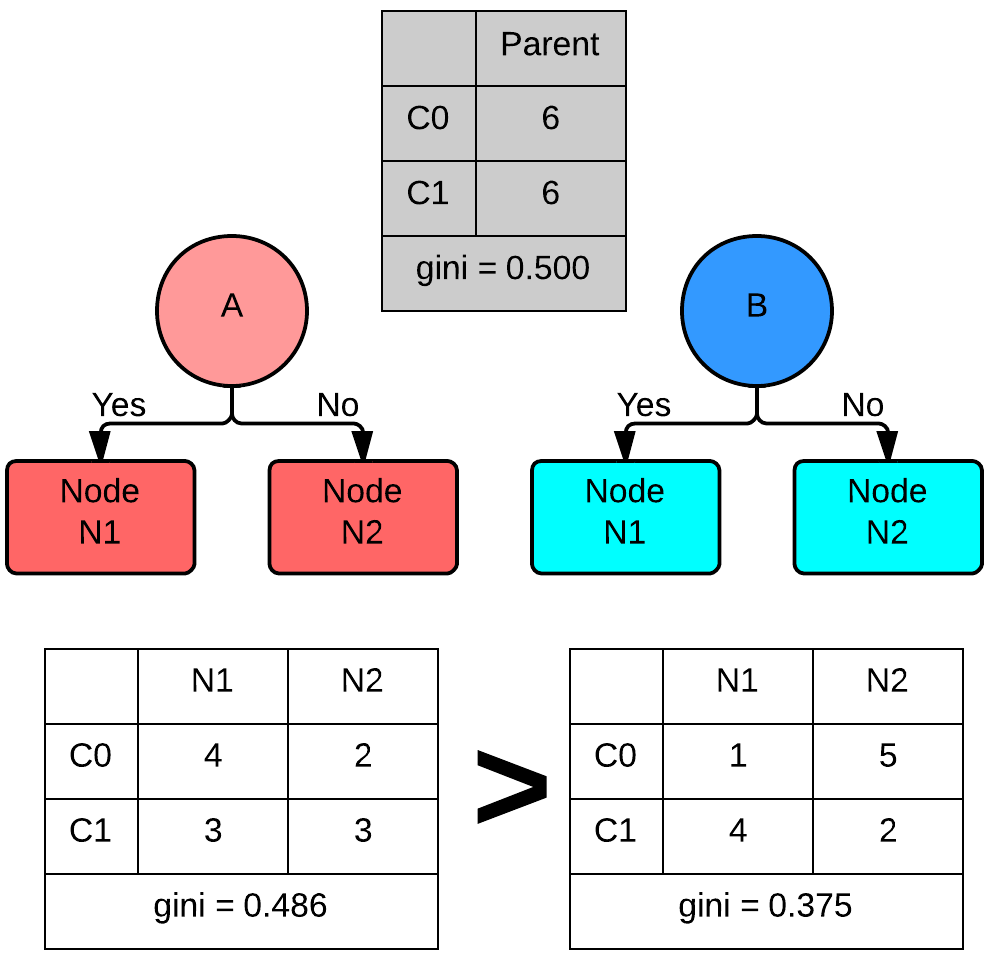
\includegraphics[scale=0.25]{pics/gini.png}
			\caption{Example of splitting binary attributes by using gini}
		\end{figure}

		{\bf Gain ratio:} in C4.5 decision tree algorithm, a splitting criterion known
		as gain ratio is used to determine the goodness of a split. The criterion is
		defined as follows:

		\begin{equation}
			Gain ratio = \frac{\Delta_{info}}{Split Info}
		\end{equation}

		\begin{equation}
			Split Info = - \sum_{i=1}^{k} P(v_{i})log_{2}P(v_{i})
		\end{equation}

		k is the total number of splits.

		\clearpage
		\section{Overfitting and undefitting}

		The errors committed by a classification model are generally divided into
		two types: {\bf training errors} and {\bf generalization errors}.
		Training error, also known as {\bf resubstitution error} or {\bf apparent error}, 
		is the number of misclassification errors committed on training records, wheras
		generalization error is expected error of the model on previously unseen records. 

		A good classification model must not only fit the training data well, it must
		also accurately classify records it has never seen before. In other words, 
		a good model must have low training error as well as low generalization error. 
		This is important because a model that fits the training data too well can 
		have a poorer generalization error than a model with a higher training error.
		Such a situation is known as model {\bf overfitting}.

		You often get high training and error rates of the model when the size of the
		tree is very small or the training set is too small. This situation is known 
		as {\bf underfitting}.

		{\bf Causes of overfitting:}
		\begin{itemize}
			\item Overfitting due to presence of noise
			\item Overfitting due to lack of representative samples
		\end{itemize}

		\subsection{Handling overfitting in decision tree induction}

		This section presents two strategies for avoiding model overfitting 
		in the context of decision tree induction. 

		{\bf Prepruning (early stopping rule):} in this approach, the tree growing
		algorithm is halted before generating a fully grown tree that perfectly
		fits the entire training data. To do this, a more restrictive stopping condition
		must be used e.g., stop expanding a leaf node when the observed gain in
		impurity measure (or improvement in the estimated generalization error) falls
		below a certain threshold. 

		{\bf Post-pruning:} in this approach, the decision tree is initially grown 
		to its maximum size. This is followed by a tree-pruning step, which proceeds
		to trim the fully grown tree in a bottom-up fashion. Trimming can be done by
		replacing a subtree with (1) a new leaf node whose class label is determined
		from the majority class of records affiliated with the subtree, or (2) the most
		frequently used branch of the subtree. 


	\clearpage
	\section{Evaluating the Performance of a Classifier}

		This section reviews some of the methods commonly used to evaluate the 
		performance og a classifier. 

		\subsection*{Holdout Method}
		In the holdout method, the original data with labeled examples is
		partitioned into two disjoint sets, called the training and the test set.
		A classification model is then introduced from the training set and its
		performance is evaluated on the test set. 

		\subsection*{Random Subsampling}
		The holdout method can be repeated several times to improve the estimation
		of a classifier's performance. This approach is known as random subsampling.
		One problem is that it does not have control over the number of times
		each record is used for testing and training. 

		\subsection*{Cross-Validation}
		An alternative to random subsampling is cross-validation. In this approach, 
		each record is used the same number of times for training and exactly once 
		for testing. To illustrate this method, suppose we partition the data into
		two equal-sized subsets. First, we choose one of the subsets for training 
		and the other for testing. We then swap the roles of the subsets so that
		the previous training set becomes the test set and vice versa. This approach
		is called a {\bf two-fold cross-validation}. The total error is obtained by summing
		up the errors for both runs. In this example, each record is exactly once 
		for training and once for testing. The {\bf k-fold cross-validation} method
		generalizes this approach by segmenting the data into k equal-sized partitions.
		During each run, one of the partitions is chosen for testing, while the rest
		of them are used for training. This procedure is repeated k times so that
		each partition is used for testing exactly once. Again, the total error is
		found by summing up the errors for all k runs. 
		A special case of the k-fold cross-validation method sets k=N, the size of 
		the data set. In this so called {\bf leave-one-out} approach, each test set 
		contains only one record. 

		\subsection*{Bootstrap}
		The methods represented so far assume that the training records are sampled
		without replacement. As a result, there are no duplicate records in the training
		and test sets. In the bootstrap approach, the training records are sampled 
		with replacement;i.e., a record already chosen for training is put back into
		the original pool or records so that it is equally likely to be redrawn. 
		It will often be the case that a bootstrap  sample size of N contains 
		about 63.2\% of the records in the original data. 
		Records that are not included in the bootstrap sample become part of the
		test set (ca 46.7\% of the original data).
		The model induced from the training set is then applied to the test set
		to obtain an estimate of the accuracy of the bootstrap sample, $e_{i}$.
		Then the sampling procedure is then repeated b times to generate b bootstrap
		samples. 

	\clearpage
	\chapter{Classification: Alternative Techniques}
	
	A {\bf Instance based} classifiers is based on the concept of "instance" and store
	the training records. It uses the training records to predict the plass label
	of unseen cases. It does not build a model in the strict sence as a decision tree. 

	{\bf Rote-learner:}
	\begin{itemize}
		\item Memorizes entire training data
		\item Performs classification only if attributes of record match
		one of the training exactly
	\end{itemize}

	In this section we will capture these algorithms: 
	\begin{itemize}
		\item Instance-based learning: k-NN
		\item Probabilistic learning: Naive Bayes
		\item Statistical learning: Support Vector Machines (SVM)
	\end{itemize}


	
	\clearpage
	\section{Nearest-Neighbor Classifiers}

		Decision tree classifier are an example of {\bf eager learner} because
		they are designed to learn a model that maps the input attributes to 
		the class label as soon as the training data becomes available. 
		An opposite strategy would be to delay the process of modeling the 
		training data until it is needed to classify the test examples.
		Techniques that employ this strategy are known as {\bf lazy learners}.

		An obvious drawback of this approach is that some test records may not
		be classified because they do not match any training example. 
		One way to make this approach more flexible is to find all the
		training examples that are relatively similar to the attribues of the
		test example. These examples are known as {\bf nearest neighbors}.

		\vspace{0.3cm}
		{\it \Large "If it walks like a duck , quacks like a duck, and looks like a duck,
		then it's probably a duck."}

		\vspace{0.3cm}

		A nearest-neighbor classifier represents each example as a data point
		in a d-dimensional space, where d is the number of attributes. 
		The k-nearest neighbors of a given example {\it z} refer to the
		{\it k} points that are close to {\it z}.
		To classify an example it uses the {\bf majority} of classes closest to the point.

		In the picture below you can see K-nearest neighbors of a record x are data 
		points that have the k smallest distance to x. In the first picture, x will
		be classified as "negative" because the majority is "negative".
		In the second picture will be classified as "positve".
		In this situation when it is a {\bf tie}, we choose randomly. 
		In the last picture	we classify x as "positive" because the majoiry is "positive"
		
		\begin{figure}[H]
			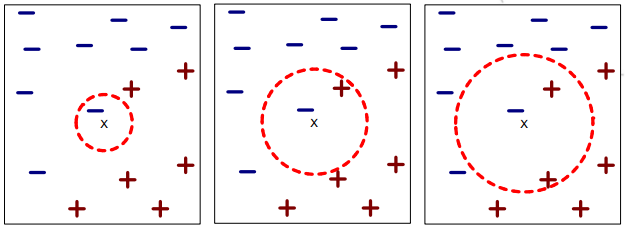
\includegraphics[width=\textwidth]{pics/knearest.png}
			\caption{1-nearest neighbor, 2-nearest neighbor and 3-nearest neighbor}
		\end{figure}

		You need to carefully pick the k because if its too small it can be close to noise
		so the classification is wrong. If the k is too big, it might happend that it
		will misclassify the test instance becuase its list of nearest neighbors may include
		data points that are located far away from its neighborhood.

		\clearpage
		\section{How to do the nearest-neighbor classifier}
		{\bf The nearest-Neighbor Classifier algorithm needs:}
			\begin{itemize}
				\item The set of stored records 
				\item Distance Metric to compute 
				\item distance between records
				\item The value of k, the number of nearest neighbors to retrieve 
			\end{itemize}
		{\bf To classify an unknown record you need to:}
			\begin{itemize}
				\item Compute distance to other training records
				\item Identify k nearest neighbors 
				\item Use class labels of nearest neighbors to determine the class 
				label of unknown record (e.g., by taking majority vote)
			\end{itemize}

		{\bf Calculate the distance between two points usin the Euclidean distance:}
		\begin{equation}
			Euclidean distance = d(p,q) = \sum_{i}^{} \sqrt{(p_{i} - q_{i})^{2}}
		\end{equation}

		\clearpage
	\section{Naive Bayes Classifier}

		In many applications the relationship between the attribute set and the class
		variable is {\bf non-deterministic}. In other words, the class label of a test
		record cannot be predicted with certainty even though its attribute set is 
		identical to some of the training examples. 

		This section presents an approach for modeling probilistic relationships
		between the attribute set and the class label. 

		Equations from probability theroy:
		\begin{equation}
			P(X,Y) = P(Y|X) \times P(X) = P(X|Y) \times P(Y)
		\end{equation}

		\begin{equation}
			P(Y|X) = \frac{P(X|Y)P(Y))}{P(X)}
		\end{equation}

		Let X denote the attribute set and Y denote the class variable. If the class variable
		has a non-deterministic relationship with the attributes, then we can treat X and Y
		as random variables and capture their relationships probabilistically using $P(Y|X)$.
		This conditional probability is also known as the {\bf posterior probability} for Y. 
		({\bf Prior probability} for Y is P(Y)).

		During the training phase, we need to learn the posterior probablities P(Y|X) for every
		combination of X an Y based on information gathered from the training data. 

		\begin{figure}[H]
			\centering
			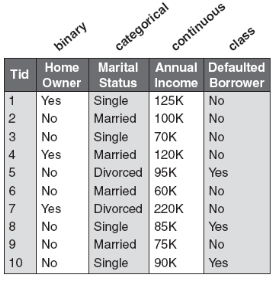
\includegraphics[scale=0.55]{pics/bayesian.png}
			\caption{Training set for predicting the loan default problem}
		\end{figure}

		Suppose we are given a test record with the following attribute set:

		X=(Home Owner = no, Marital Status = Married, Annual Income = 120K).

		To classify the record, we need to compute the posterior probabilities
		$P(Yes|X)$ and $P(No|X)$ based on the information available in the training data.
		If $P(Yes|X) > P(No|X)$, then the record is classified as Yes, otherwise it is classified
		as No. 

		When comparing the posterior probabilities for different values of Y, the denominator term
		{\bf P(X)}, is always {\bf constant}, and thus, can be ignored. 
		The prior probability {\bf P(Y)} can be easily estimated from the training set by computing
		the fraction of training records that belong to each class.	

		A naive Bayes classifier estimates the class-conditional probability by assuming 
		that the attributes are {\bf conditionally independent}, given the class variable y. 
		The assumption of conditionally independence of the attributes is the reason why P(X)
		can be ignored!

		\subsection*{Example: Play Tennis data}

		\begin{figure}[H]
			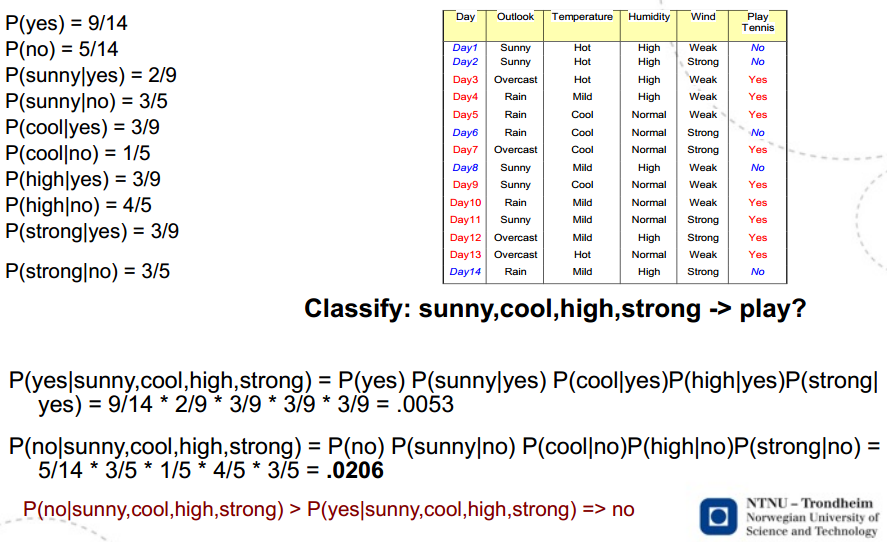
\includegraphics[width=\textwidth]{pics/examplenaive.png}
		\end{figure}

		\subsection{Estimating Conditional Probabilities for Continuous Attributes}

			There are two ways to estimate the class-conditional probabilities for 
			continuous attributes:

			\subsection*{1) Discretization}

				We can discretize each continuous attribute and then replace the continuous
				attribute value with its corresponding discrete interval. This approach
				transforms the continuous attributes into ordinal attributes. 
				Be aware of the interval! To small or big interval can make a huge error in
				the classification. 

			\subsection*{2) Gaussian Distribution}

				We can assume a certain form of probability distribution for the continuous
				variable and estimate the parameters of the distribution using the training data. 
				A {\bf Gaussian distribution} is usually chosen to represent the class-conditional
				probability for continuous attributes. The distribution is characterized by two 
				parameters, its mean, $\mu$, and variance, $\sigma^{2}$.
				for each class label $y_{j}$, the class-conditional probability for attribute $X_{i}$ is:

				\begin{equation}
					P(X_{i} = x_{i}|Y = y_{j}) = \frac{1}{\sqrt{2\pi} \sigma_{ij}} 
					exp^{-\frac{(x_{i}-\mu_{ij})^{2}}{2\sigma^{2}_{ij}}}
				\end{equation} 

				The parameter $\mu_{ij}$ can be estimated based on the sample mean of $X_{i}$ 
				($\overline{x}$) for all training records that belong to the class $y_{j}$.
				Similary, $\sigma^{2}_{ij}$ can be estimated from the sample variance ($s^{2}$)
				of such training records. 

				Consider the example for figure 5.2 with training set for loan. We will look at the
				continuous attribute annual income.  
				The sample mean and variance for this attribute with respect to the class label No
				are:

				\begin{equation}
					\overline{x} = \frac{125 + 100 + 70 + .... + 75}{7} =110
				\end{equation}

				\begin{equation}
					s^{2} = \frac{(125-110)^{2} + (100-110)^{2} + .... + (75-110)^{2}}{7-1} = 2975
				\end{equation}

				\begin{equation}
					s = \sqrt{2975} = 54.54
				\end{equation}

				Given a sample record given earlier:

				X=(Home Owner = no, Marital Status = Married, Annual Income = 120K)

				we can compute its class-conditional probability as follows:

				\begin{equation}
					P(Income = 120|No) = \frac{1}{\sqrt{2\pi}(54.54)}
					exp^{-\frac{(120-110)^{2}}{2*2975}} = 0.0072
				\end{equation}

				In order to predict the class label of record X, we need to compute the 
				posterior probabilities $P(No|X)$ and $P(Yes|X)$

				\begin{figure}[H]
					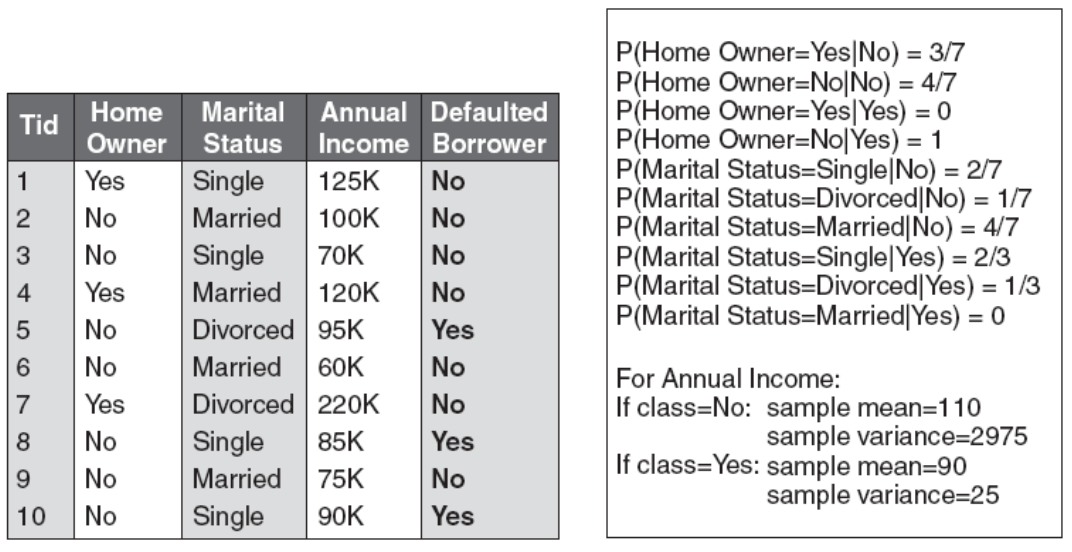
\includegraphics[width=\textwidth]{pics/example.png}
				\end{figure}

				\begin{equation}
				\begin{split}
					P(X|No) = P(Home Owner = No|No) \times P(Status = Married|No) \\
					\times P(Annual Income = 120K|No)
					= \frac{4}{7} \times \frac{4}{7} \times 0.0072 = 0.0024
				\end{split}
				\end{equation}

				\begin{equation}
				\begin{split}
					P(X|Yes) = P(Home Owner = No|Yes) \times P(Status = Married|Yes) \\
					\times P(Annual Income = 120K|Yes)
					= 1 \times 0 \times 1.2 \times 10^{-9} = 0
				\end{split}
				\end{equation}

				\begin{equation}
					P(X|No) > P(X|Yes) \rightarrow X has\:the\:class\:label\:No
				\end{equation}

		\subsection{Problems with naive bayes}

			If you look at the previous example, the calculation of $P(X|Yes)$ was zero
			because one of the attributes had a count of 0. A problem is when we only have 
			a small set of training data, then we probably could get a situation where
			$P(X|Yes)$ = 0 and $P(X|No)$ = 0. What to do now?!

			This problem can be addressed by using the {\bf m-estimate} approach for 
			estimating the conditional probabilities. 

			\begin{equation}
				P(x_{i}|y_{j}) = \frac{n_{c} + mp}{n+m}
			\end{equation}

			where n is the total number of instances from class $y_{j}$, 
			$n_{c}$ is the number of training examples from class $y_{j}$ that takes on the 
			value $x_{i}$, m is a parameter known as the equivalent samle size, and p is a 
			user-specified parameter.

			We can also use the {\bf Laplace} equation:
			\begin{equation}
				P(x_{i}|Y) = \frac{n_{c} +1}{n + c}
			\end{equation}

			where c is the number of classes.

			In the example above we got $P(Status = Married|Yes) = 0$. Using the m-estimate
			with m = 3 and p = 1/3, the conditional probability is no longer zero:

			$P(Marital Status = Married|Yes) = (0+3 \times 1/3)/(3+3)$


		\subsection{Characteristics of Naive Bayes Classifiers}

			\begin{itemize}
				\item They are robust to isolated {\bf noice points} becuase such points are 
				averaged out when estimating conditional probabilities from data. 
				Naive Bayes classifiers can also handle missing values by ignoring the
				example during model building and classification.
				\item They are robust to {\bf irrelevant attributes}. If $X_{i}$ is an irrelevant
				attribute, then $P(X_{i}|Y)$ becomes alomst uniformly distributed. 
				\item {\bf Correlated attributes} can degrade the performance of naive Bayes 
				classifiers because the conditional independence assuption no longer holds 
				for such attributes. 
			\end{itemize}

		\subsection{Bayes Error Rate}

			\begin{equation}
				(\frac{\hat{x} - \overline{x}_1}{s}) = (\frac{\hat{x} - \overline{x}_2}{s} )
			\end{equation}

			Solve this equation for $\hat{x}$ and use it in the next equation for calculating
			the {\bf Bayes error rate}:

			\begin{equation}
				Error = \int_{0}^{\hat{x}} P(Y_{1}|X) dX + \int_{\hat{x}}^{\infty} P(Y_{2}|X)) dX
			\end{equation}

	\section{Support Vector Machine (SVM)}

		Finds a linear {\bf hyperplane} (decision boundray) that will separate the data. 
		The classifier must choose one of these hyperplanes to represent its decision
		boundery, based on how well they are expected to performm on test examples. 

		\begin{figure}[H]
			\subfigure{
				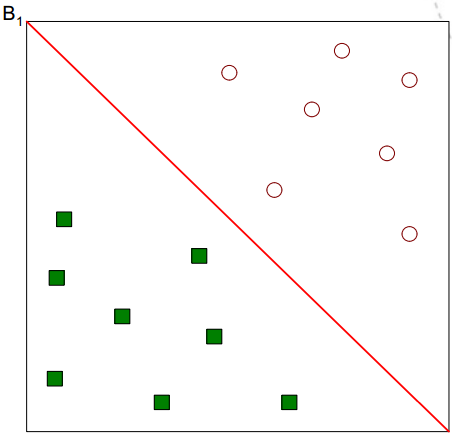
\includegraphics[scale=0.25]{pics/svm1.png}
			}
			\subfigure{
				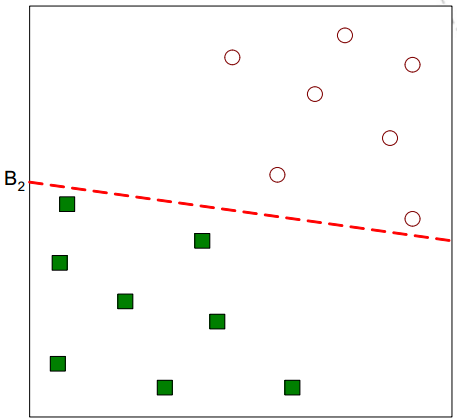
\includegraphics[scale=0.25]{pics/svm2.png}
			}
			\subfigure{
				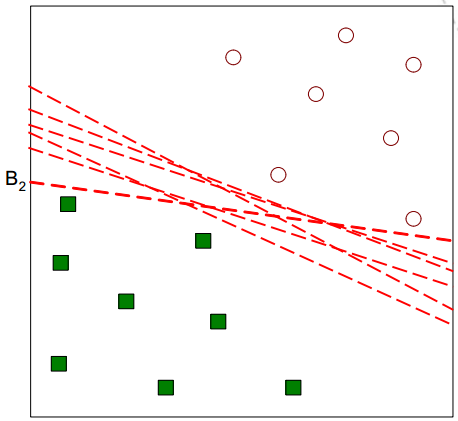
\includegraphics[scale=0.25]{pics/svm3.png}
			}
			\caption{B1, B2, and other solutions}
		\end{figure}

		Which one is better?

		\begin{figure}[H]
			\subfigure{
				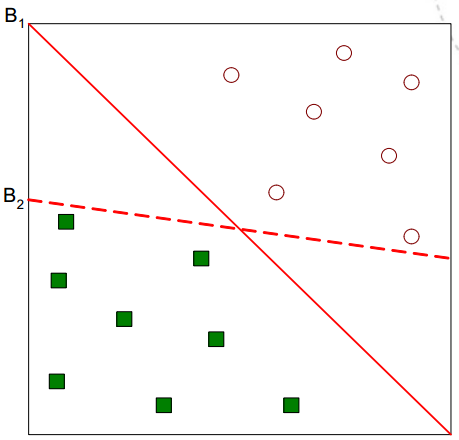
\includegraphics[scale=0.4]{pics/svm4.png}
			}
			\subfigure{
				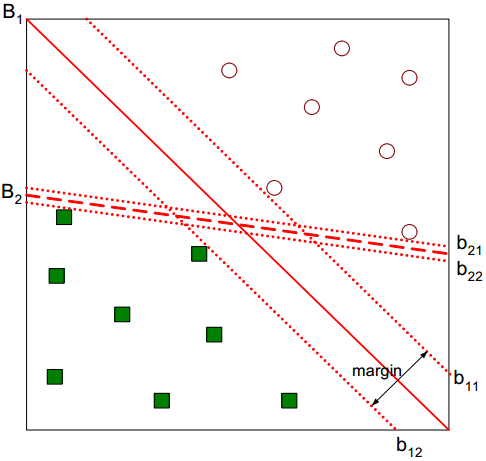
\includegraphics[scale=0.4]{pics/svm5.png}
			}
			\caption{B1 and B2, and the magins}
		\end{figure}

		We want to find hyperplane that maxximizes the margin, therefore we would pick B1. 



	\clearpage
	\chapter{Association Analysis: Basic Concepts and Algorithms}

	This chapter presents a methodology known as {\bf association analysis},
	which is useful for discovering interesting relationships hidden in large
	data sets, such as shopping basket transactions. 
	The uncovered relationships can be represented in the form of 
	{\bf association rules} or sets of {\bf frequent items}. 

	\clearpage
	\section{Problem Definition}

	This section reviews the basic termonology used in association analysis.

		\subsection*{Binary representation} 
		market basket data can be represented in a binary
		format as shown below. Each row correspond to a transaction (TID = transactio ID)
		and each column correspond to an item. A item in a transaction have the value
		"1" if the item is present in the transaction, otherwise it is "O".
		Because the presence of an item in a transaction is often considered more
		important than its absence, an item is an {\bf asymmetric binary value}.

		\begin{figure}[H]
		\centering
			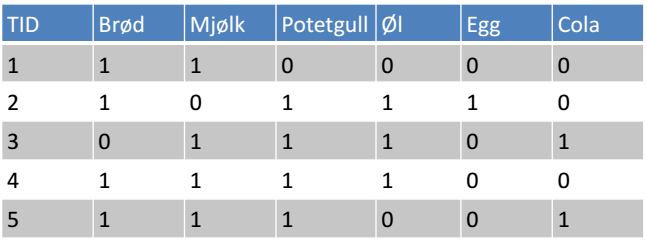
\includegraphics[scale = 0.4]{pics/binary.png}
			\caption{Binary representation of transaktions from market basket data}
		\end{figure}

		\subsection*{Itemset and support count} 
		Let $ I = \{i_{1}, i_{2}, ...., i_{d}\}$ be the
		set of all items in a market basket data and $ T = \{t_{1}, t_{2},....,t_{N}\}$
		be the set of all transactions. Each transaction $t_{i}$ contains a subset of items
		chosen from I. In assiciation analysis, a collection of zero or more items
		is termed an {\bf itemset}. If an itemset contains k items, it is called a {\bf k-itemset}.
		The {\bf transaction width} is defined as the number of items present in a transaction.
		An important property of an itemset is its {\bf support count}, which refers to the 
		number of transactions that contain a particular itemset. 

		\subsection*{Association rule and confidence} 
		An association rule is an implication expression of
		the form $X \rightarrow Y$, where X and Y are disjoint itemsets, i.e., $X \cap Y = \emptyset$.
		The strength of an association rule can be measured in terms of {\bf support} and 
		{\bf confidence}. Support determines how often a rule is applicable to a given data
		set, while confidence determines how frequently items in Y appear in transactions that
		contains X. 

		\begin{equation}
			Support, s(X \rightarrow Y) = \frac{\sigma (X \cup Y)}{N}
		\end{equation}

		\begin{equation}
			Confidence, c(X \rightarrow Y) = \frac{\sigma(X \cup Y)}{\sigma(X)}
		\end{equation}

		\clearpage

		\subsection*{Why use support and confidence?}

		Support is an iportant measure because a rule that has very low support may occur simply
		by chance, or is likely to be uninteresting from a business perspective. 
		Confidence, on the other hand, measures the realiability of the inference made by a rule.
		For a given rule {\bf X $\Rightarrow$ Y}, the higher the confidence, the more likely it 
		is for Y to be present in transactions that contain X. 

		\subsection*{Example support and confidence}
		The number is from figure 6.1. We will calculate the support and confidence for the 
		association rule {\bf \{Mjølk, Potetgull\} $\Rightarrow$ \{Øl\}}. \\
		\{Mjølk, Potetgull, Øl\} appear in 2 of the transactions and \{Mjølk, Potetgull\} is 
		appear in 3 of the transactions. The total number of transactions is 5.   
		
		\begin{equation}
			s = \frac{\sigma(Mjølk,Potetgull, Øl)}{Number of transactions} = \frac{2}{5} = 0.4
		\end{equation}
		\begin{equation}
			c = \frac{\sigma(Mjølk, Potetgull, Øl)}{\sigma(Mjølk, Potetgull)} =  \frac{2}{3} = 0.67
		\end{equation}

		\subsection*{Minsup and minconf threshold}
		Given a set of transactions T, find all the rules having support $\geq$ minsup and \\
		confidence $\geq$ minconf, where minsup and minconf are the corresponding support
		and confidence thresholds. 

		A brute-force apporach for mining association rules is to compute the support and
		confidence for every possible rule. This approach is prohibittively expensive!
		Therefore, a common strategy is to decompose the problem into two major subtasks:

		\begin{enumerate}
			\item {\bf Frequent Itemset Generation,} whose objective is to find all the 
			itemsets that satisfy the minsup threshold. These itemsets are called 
			frequent itemsets. 
			\item {\bf Rule generation,} whose objective is to extract all the high-confidence
			rules from the frequent itemsets found in the previous step. These rules
			are called {\bf strong rules}.
		\end{enumerate}

	\clearpage 
	\section{Frequent Itemset Generation}

		A lattice structure can be used to enumerate the list of all possible itemsets.
		Figure 6.2 shows an itemset lattice for I = \{a,b,c,d,e\}. The lattice shows
		all possible itemsets, also called {\bf candidate itemsets}. To calculate
		the support count for every candidate itemsets, we need to compare each candidate
		against every transaction.

		\begin{figure}[H]
			\centering
			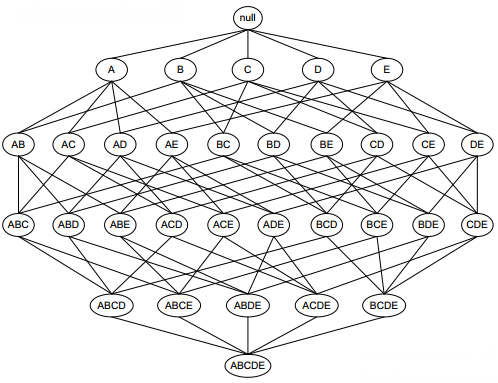
\includegraphics[scale=0.5]{pics/lattice.png}
			\caption{An itemset lattice}
		\end{figure}

		This method have a hight computational compleexity. There are several ways to reduce 
		the computitional complexity for frequent itemset generation. 

		\begin{enumerate}
			\item {\bf Reduce the number of candidate itemsets (M):} the {\it Apriori}
			princible in the next section is an very effective way to eliminate
			some of the candidate itemsets without counting their support values. 
			\item{\bf Reduce the number of comparisons:} Instead of matching each candidate
			itemset against every transaction, we can reduce the number of 
			comparisons by using more advanced data structures, either to store the
			candidate itemsets or to compress the data set. 
		\end{enumerate}

	\clearpage
	\section{The Apriori Principle}

		{\bf Apriori principle:} {\it If an itemset is frequent, then all of its subsets must also be frequent}.

		\begin{figure}[H]
			\centering
			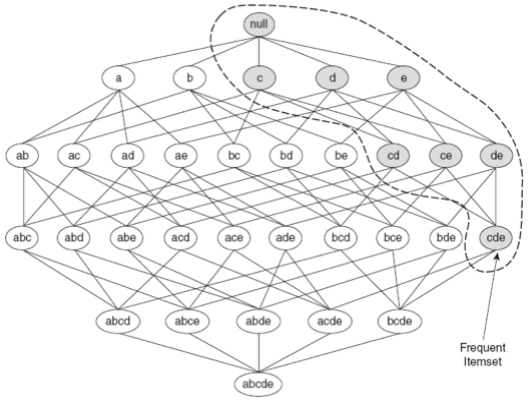
\includegraphics[scale=0.5]{pics/lattice3.png}
			\caption{Apriori principle: the itemset cde + all of its subsets is a frequent itemset}
		\end{figure}

		\begin{figure}[H]
			\centering
			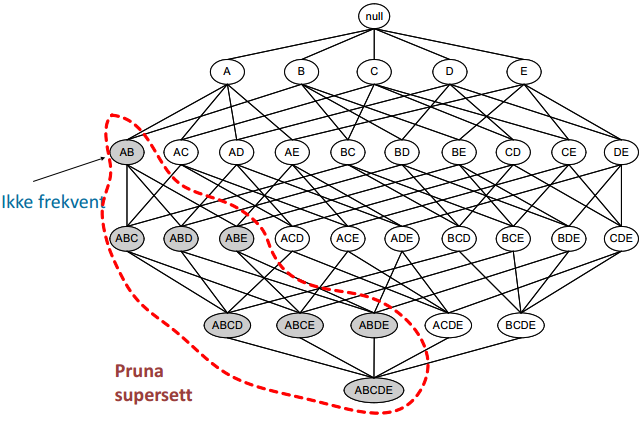
\includegraphics[scale=0.5]{pics/lattice4.png}
			\caption{Apriori principle: the itemset AB is infrequent, then all of its supersets must be infrequent}
		\end{figure}

	\clearpage

	\section{Apriori Algorithm}

		Let $C_{k}$ denote the set of candidate k-itemsets and $F_{k}$ denote the set of frequent 
		k-itemsets:

		\subsection*{The frequent itemset generation part of the Apriori algorithm}
		\begin{itemize}
			\item The algorithm initially makes a single pass over the data set to determine
			the support of each item. Upon completion of this step, the set of all frequent
			1-itemsets, $F_{1}$, will be known.
			\item Next, the algorithm will iteratively generate new candidate k-itemsets
			using the frequent (k-1)-itemsets found in the previous iteration. Candidate
			generation is implemented using a function called apriorigen.
			\item To count the support of the candidates, the algorithm needs to make 
			an additional pass over the data set. The subset function is used to determine
			all the candidate itemsets in $C_{k}$ that are contained in each transaction t.
			\item After counting their supports, the algorithm eliminates all candidate
			itemsets whose support counts are less than minsup.
			\item The algorithm terminates when there are no new frequent itemsets generated,
			i.e., ($F_{k} = \emptyset$).
		\end{itemize}

		\subsection*{Apriori-gen function}
		\begin{itemize}
			\item {\bf Candidate Generation:} this operation generates new candidate
			k-itemsets based on the frequent (k-1)-itemsets found in previous iteration.
			\item {\bf Candidate Pruning:} this operation eliminates some of the candidate
			k-itemsets using the support-based pruning strategy
		\end{itemize}

		\begin{figure}[H]
			\centering
			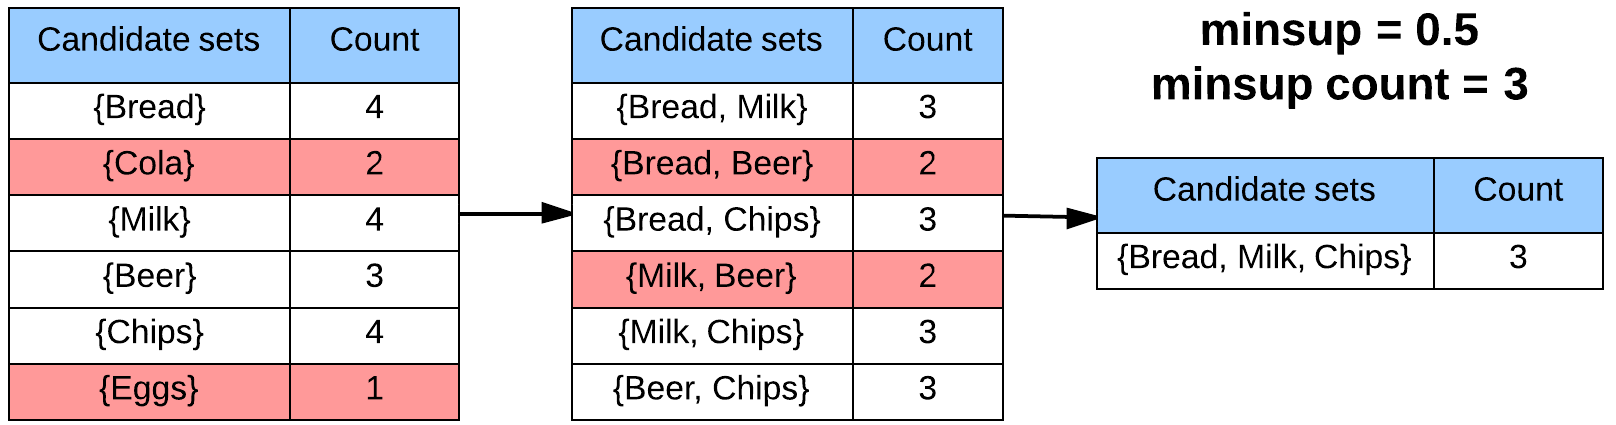
\includegraphics[width=\textwidth]{pics/apriori.png}
			\caption{Itemset generation with pruned itemsets in red}
		\end{figure}

		\subsection*{Requirements for an effective candidate generation procedure}

		\begin{enumerate}
			\item It should avoid generating too many unnecessary candidates.
			\item It must ensure that the candidate set is complete, i.e., no frequent
			itemsets are left out by the candidate generation procedure. 
			\item It should not generate the same candidate itemset more than once.
		\end{enumerate}

		\clearpage
		\section{Apriori Candidate generation procedures}

			\subsection{Brute-Force Method}
				The brute-force method considers every k-itemsets as a potential candidate and then 
				applies the candidate pruning step to remove any unnecessary candidates. 

			\subsection{$F_{k-1} \times F{1}$ Method}
				An alternative method for generation is to extend each frequent (k-1)-itemset with 
				other frequent items. This method can generate duplicate candidates. One way of
				avoid generating duplicate candidates is by ensuring that the items in each frequent 
				itemset are are kept strted in their lexicographically larger than the items in X. 
				For examplel, the itemset \{Bread, Diapers\} can be argumented with \{Milk\}
				since Milk is lexiicographically larger than Bread and Diapers. However, we
				should not augment \{Bread, Diapers\} with \{Bread\} nor \{Bread, Milk\} with 
				\{Diapers\} because they violate the lexocographic ordering condition. 
 
			\subsection{$F_{k-1} \times F_{k-1}$ Method}
				The candidate generation procedure in the apriori-gen function merges a pair of 
				frequent (k-1)-itemsets only if their first k-2 items are identical. 
				Let A = \{$a_{1}, a_{2},...,a_{k-1}$\} and B = \{$b_{1}, b_{2},...,b_{k-1}$\}
				be a pair of frequent (k-1)-itemsets. A and B are merged if they satisfy the following
				conditions:

				$a_{i} = b_{i} (for i =1, 2,..., k-2)$ and $a_{k-1} \neq b_{k-1}$

				The frequent itemsets \{Bread, Diapers\} and \{Bread, Milk\} are merged to form a 
				candidate 3-itemset \{Bread, Diapers, Milk\}. The algorithm does not have to merge
				\{Beer, Diapers\} with \{Diapers, Milk\} because the first item in both itemsets is
				different. Indeed, if \{Beer, Diapers, Milk\} is a viable candidate, it would have been
				obtained by merging \{Beer, Diapers\} with \{Beer, Milk\}.
				
				\begin{figure}[H]
					\centering
					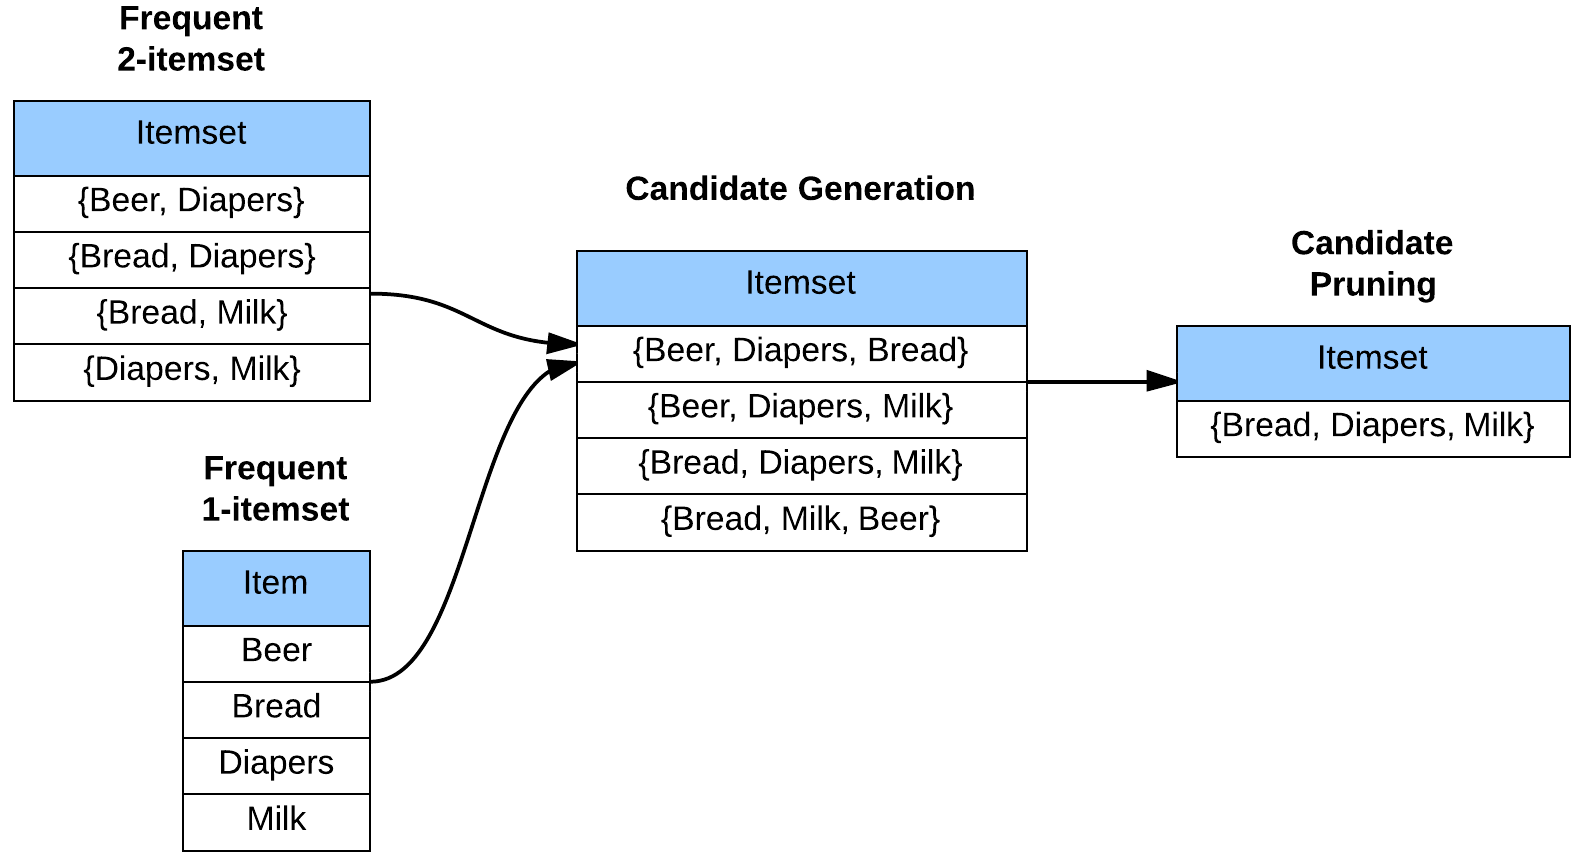
\includegraphics[width=\textwidth]{pics/apriori2.png}
					\caption{$F_{k-1} \times F{1}$ illustration}
				\end{figure}

				\begin{figure}[H]
					\centering
					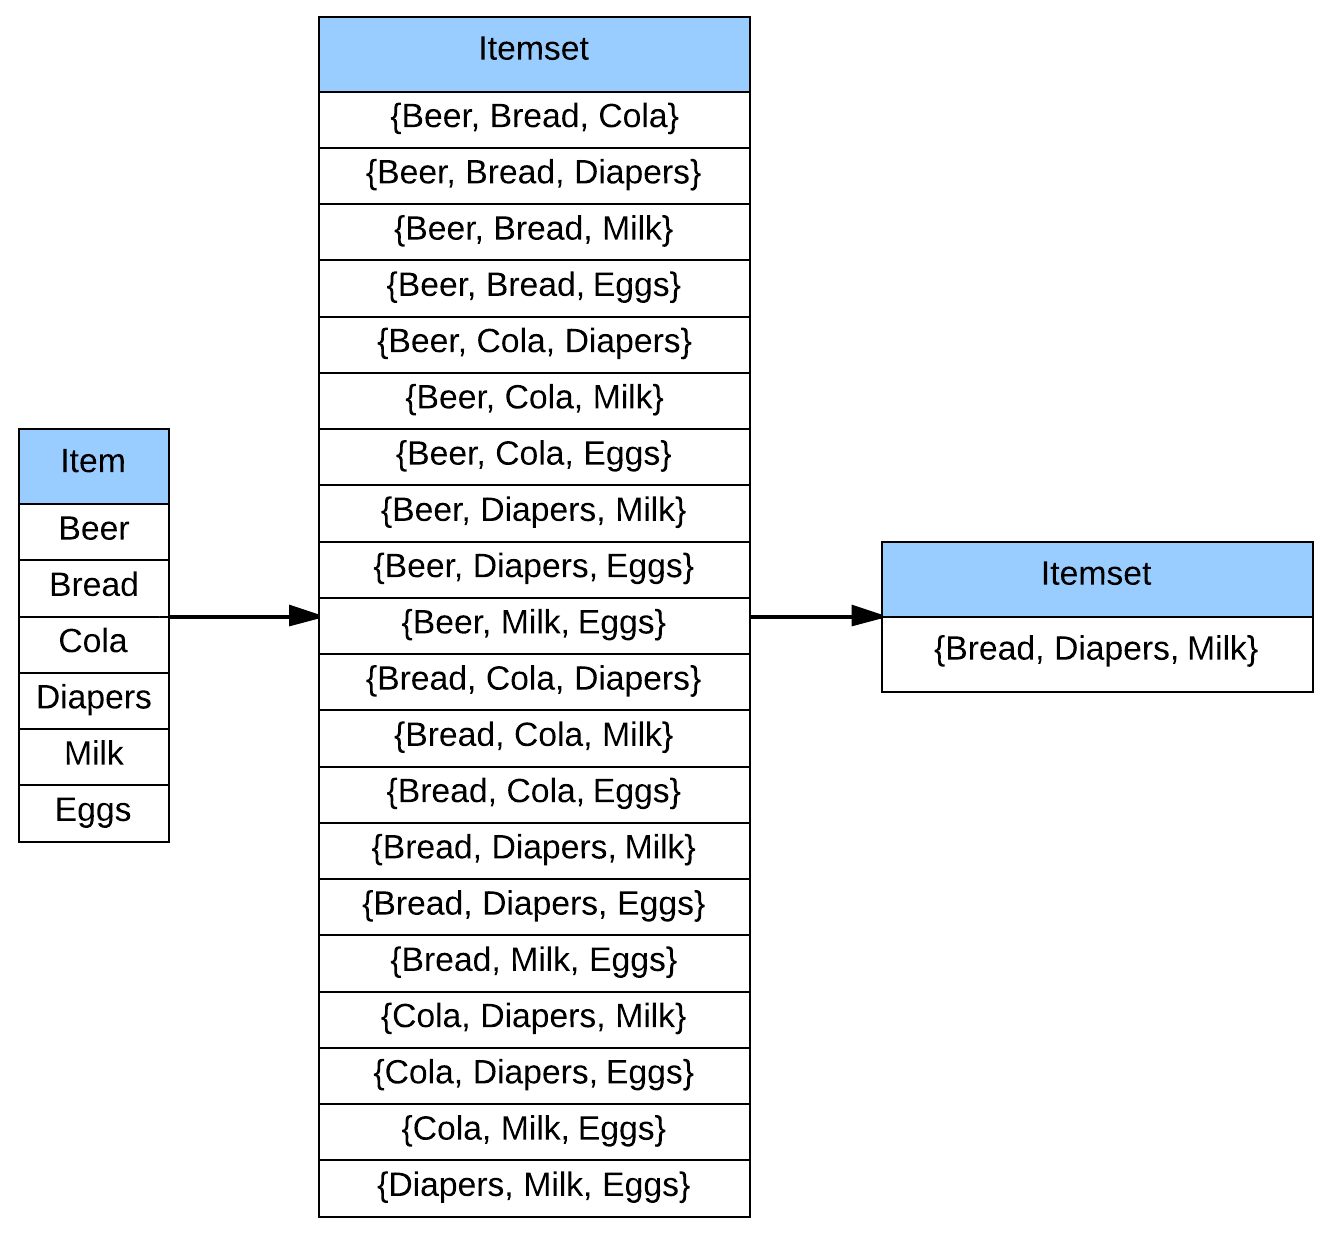
\includegraphics[scale=0.2]{pics/apriori1.png}
					\caption{Brute-Force illustration}
				\end{figure}

				\begin{figure}[H]
					\centering
					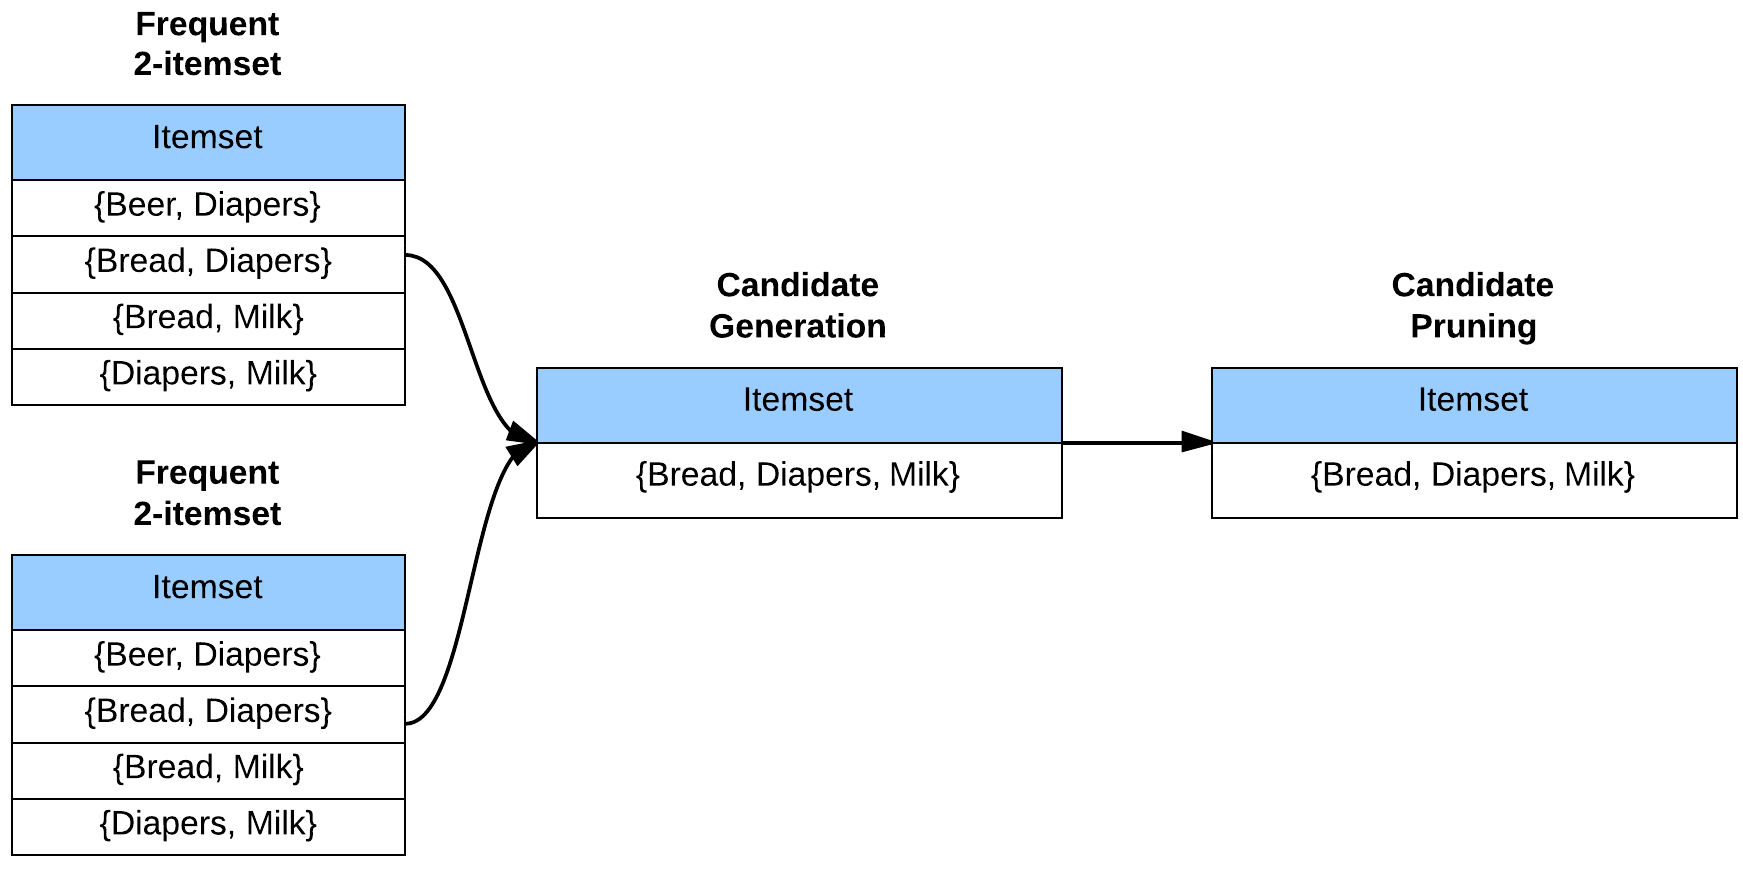
\includegraphics[width=\textwidth]{pics/apriori3.png}
					\caption{$F_{k-1} \times F_{k-1}$ illustration}
				\end{figure}

	\clearpage
	\section{Support Counting}

	Support counting is the process of determining the frequency of occurance for every candidate itemset
	that survives the candidate pruning step of the apriori-gen function. 

	One approach for doing this is to compare each transaction against very candidate itemset and 
	to update the support counts of candidates contained in the transaction. 

	An alternative approach is to enumerate the itemsets contained in each 
	transaction and use them  to update the support counts of their respective candidatee itemsets.
	
		\begin{figure}[H]
		\centering
		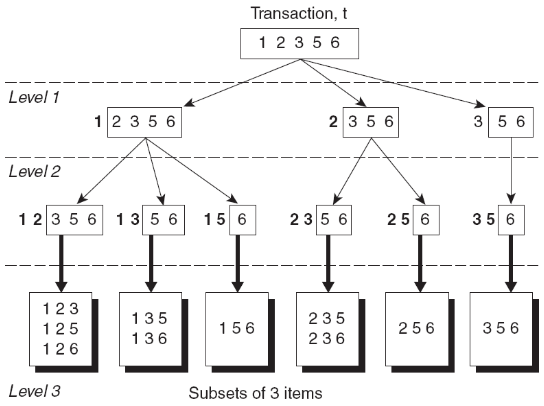
\includegraphics[scale=0.5]{pics/enumerateSubsets.png}
		\caption{Enumerating subsets of three items from a transaction t}
		\end{figure}

	In the Apriori algorithm, candidate itemsets are partitioned into different buckets and stored
	in a hash tree. During support counting, itemsets contained in each transaction are also hashed 
	into their appropriate buckets. That way, instead of comparing each itemset in the transaction 
	with every candidate itemset, it is matched only against candidate itemsets that belong to the 
	same bucket. 

		\begin{figure}[H]
			\centering
			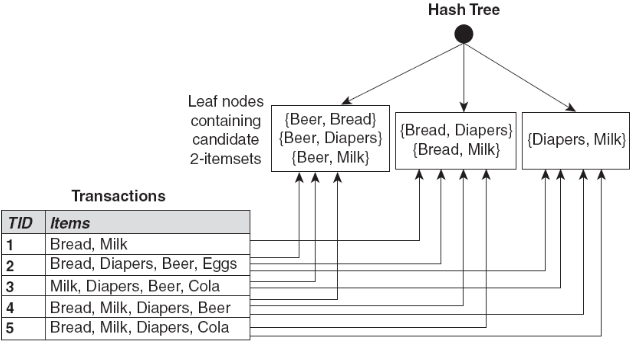
\includegraphics[scale=0.5]{pics/supportCount.png}
			\caption{Counting support of itemsets using hash structure}
		\end{figure}

		\begin{figure}[H]
			\centering
			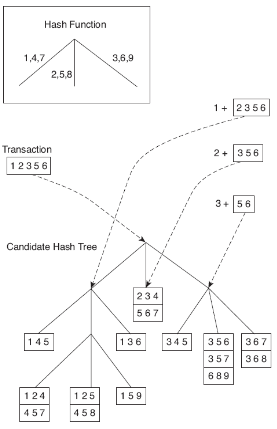
\includegraphics[scale=0.6]{pics/hash.png}
			\caption{Hasing a transaction at the root node of a hash tree}
		\end{figure}

	\section{Computational Complexity}

	The computational complexity of the apriori algorithm can be affected by the following factors:

		\begin{itemize}
			\item {\bf Support Threshold:} lowering the support threshold often results in more
			itemsets being declared as frequent. More frequent itemsets gives more comparisions in
			the algorithm.
			\item {\bf Number of items (Dimensionality):} As the number of items increases, more
			space will be needed to store the support counts of items. 
			\item {\bf Number of transactions:} since the apriori algorithm makes repeated passes
			over the data set, its run time increases with a large number of transactions. 
			\item {\bf Average transaction width:} this affects the Apriori algorithm in two ways.
			First, the maximum  size of frequent itemsets tends to increase as the 
			average transaction width increases. As a result, more candiadate itemsets must be
			examined during candidate generation and support counting.
			Second, as the transaction width increases. more
			itemsets are contained in the transaction. This will increase the number of hash 
			tree traversals performed during support counting.
			\item {\bf Generation of frequent 1-itemsets:} for each transaction, we need to 
			update the support count for every item present in the transaction.
			\item {\bf Candidate generation} 
			\item {\bf Support counting} 
		\end{itemize}




	\clearpage
	\section{Rule Generation}

		This section describes how to extract association rules efficiently from a given 
		frequent itemset. 

		{\bf Theorem:} {\it If a rule X $\rightarrow$ Y - X does not satisfy the confidence
		threshold, then any X' $\rightarrow$ Y - X', where X' is a subset of X, must not satisfy
		the confidence threshold as well.}

		\subsection*{Rule generation in Apriori Algorithm}

		The Apriori algorithm uses a level-wise approach for generating association rules, 
		where each level corresponds to the number of items that belong to the rule 
		consequent. Initially, all the high-confidence rules that have only one item
		in the rule consequent are extracted. These rules are then used to generate
		new candidate rules.

		{\bf Example:} if \{acd\} $\rightarrow$ \{b\} and \{abd\}$\rightarrow$\{c\} are
		high-confidence rules, then the candidate rule \{ad\} $\rightarrow$ \{bc\} is
		generated by merging the consequents of both rules. 
		
		Suppose the confidence for \{bcd\} $\rightarrow$ \{a\} is low. All the rules
		containing item a in its consequent, including \{cd\} $\rightarrow$ \{ab\},
		\{bd\} $\rightarrow$ \{ac\}, \{bc\} $\rightarrow$ \{ad\}, and \{d\} $\rightarrow$ \{abc\}
		can be discarded.

		\begin{figure}[H]
			\centering
			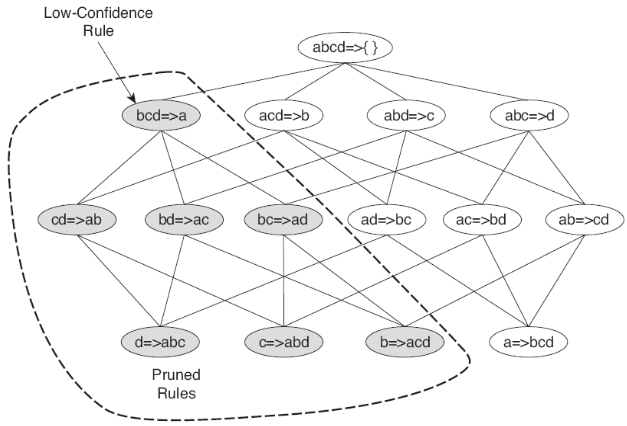
\includegraphics[width=\textwidth]{pics/prune.png}
			\caption{Pruning of association rules using the confidence measure}
		\end{figure}

	\clearpage
	\section{Compact Representation of Frequent Itemsets}
		In practice, the number of frequent itemsets produced from a transaction data set
		can be very large. It is useful to identify a samll representative set of itemsets
		from which all other frequent itemsets can be derived. 
		Two such representations are presented in this section in the form of maximal and
		closed frequent itemsets.

		\subsection{Maximal Frequent Itemsets}

		{\bf Maximal Frequent Itemsets:} a maximal frequent itemset is defined as a frequent
 		itemset for which none of its immidiate supersets are frequent.

 			\begin{figure}[H]
 				\centering
 				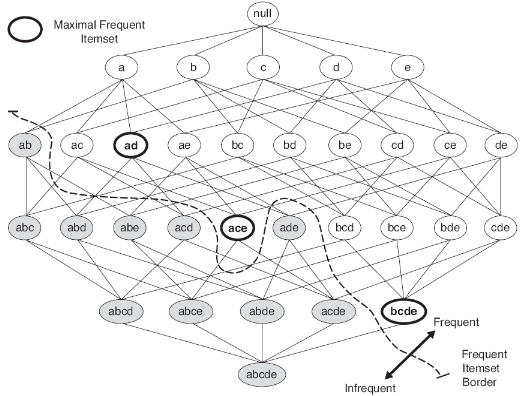
\includegraphics[scale=0.6]{pics/maximal.png}
 			\end{figure}

 		Maximal frequent itemsets form the smallest set of itemsets from which all frequent 
 		itemsets can be derived. For example, the frequent itemsets shown in figure ...
 		can be divided into two groups:

 		\begin{itemize}
 			\item Frequent itemsets that begin with item a and that may contain items
 			c, d, or e. This group includes itemsets such as \{a\}, \{a,c\}, \{a,d\},
 			\{a,e\}, and \{a,c,e\}.
 			\item Frequent itemsets that begin with items b, c, d or e. This group
 			includes itemsets such as \{b\}, \{b,c\}, \{c,d\}, \{b,c,d,e\}, etc.
 		\end{itemize}

 		\clearpage
 		\subsection{Closed Frequent Itemsets} 

 			Closed itemsets provide a minimal representation of itemsets without losing
 			their support information.

 			{\bf Closed Itemset:} {\it An itemset X is closed if none of its immidiate supersets has
 			exactly the same support count as X. }

 			{\bf Closed Frequent Itemsets:} {\it An itemset is a closed frequent itemset
 			if it is closed and its support is greater than or eaqual to minsup.}
 			\begin{figure}[H]
 				\centering
 				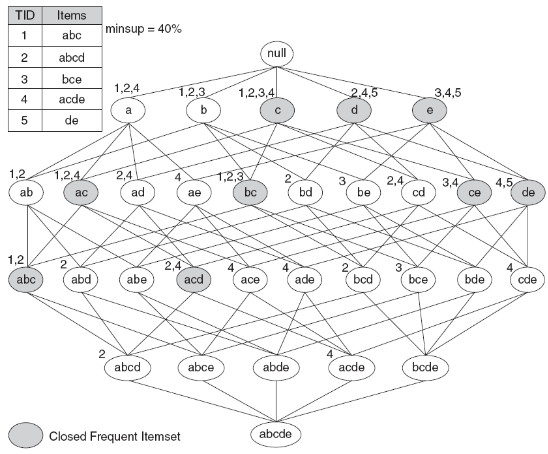
\includegraphics[scale=0.6]{pics/closed.png}
 				\caption{An example of the closed frequent itemsets (minsup = 40\%)}
 			\end{figure}

 			In figure 6.13 we have associated each node (itemset) in the lattice with a list
 			of its corresponding transaction IDs. For example, since the node \{b,c\} is
 			associated with transaction IDs 1,2 and 3, its support count is equal to 3. 

 			\begin{figure}[H]
 				\centering
 				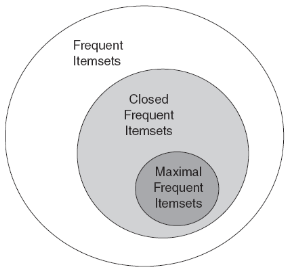
\includegraphics[scale=0.5]{pics/relationship.png}
 				\caption{Relationships among frequent, maximal frequent, and closed maximal frequent itemsets}
 			\end{figure}


 	\section{Alternative Methods for Generating Frequent Itemsets}

 		Several alternative methods have been developed to overcome these limitations of the,
 		and improve upon the efficiency of the Apriori algorithm. The following is a high-level
 		description of these methods:

 		\subsection{Traversal of Itemset Lattice}

 		Different search strategies in  traversal on a itemset lattice:
 		
 		{\bf General-to-specific vs. Specific-to-general:} The apriori 
 			algorithm uses a general-to-specific search strategy, where pairs of
 			frequent (k-1)-itemsets are merged to obtain candidate k-itemsets.
 			The difference between these is wether you start the search on the top
 			or on the bottom. You can use a {\bf bidirectional} where you start in both
 			ends and meets in the middle. 

 			\begin{figure}[H]
 				\centering
 				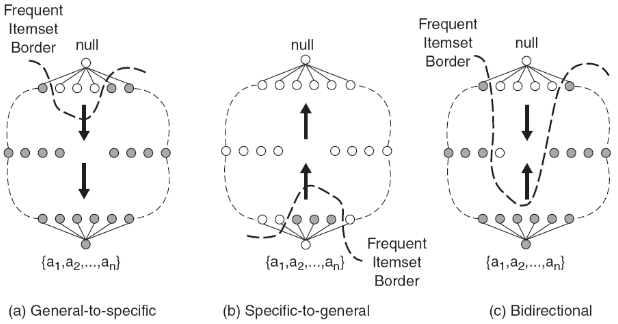
\includegraphics[scale=0.5]{pics/traversal.png}
 				\caption{General-to-specific, Specific-to-general, and bidirectional search}
 			\end{figure}
 		
 		{\bf Equivalence Clases:} Another way to envision the traversal is to
 			first partition the lattice into disjoint groups of nodes (or equivalence classes).
 			A frequent itemset generation algorithm searches for frequent itemsets within
 			a particualar equivalence class before moving to another equivalence class. 
 			Equivalence classes can be defined according to the {\bf prefix} of {\bf suffix} labels of 
 			an itemset. In this case, two itemsets belong to the same equivalence class if 
 			they share a common prefix or suffix of length k.

 			\begin{figure}[H]
 				\centering
 				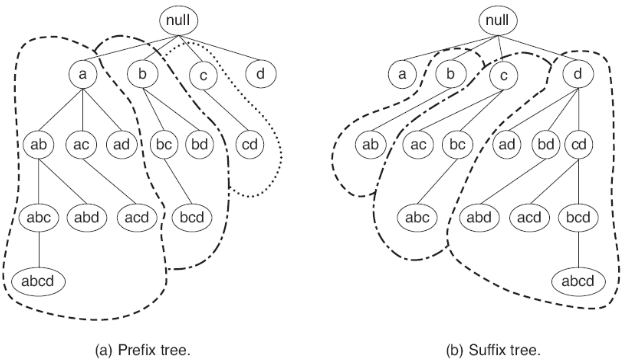
\includegraphics[scale=0.36]{pics/equvivalence.png}
 				\caption{Equvivalence classes based on the prefix and suffix labels of itemsets}
 			\end{figure}

 		{\bf Breadth-First vs. Depth-First:} The Apriori algorithm traverses the lattice in a breadth-first
 		manner. It first discovers all the frequent 1-itemsets, followed by the frequent 2-itemsets,
 		and so on, until no new frequent itemsets are generated. The itemset lattice ccan also be
 		traversed in a depth-first manner.

 		\begin{figure}[H]
 				\centering
 				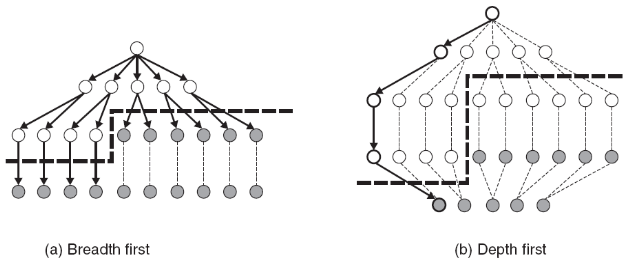
\includegraphics[scale=0.5]{pics/bfdf.png}
 				\caption{Breadth-first and depth-first straversals}
 		\end{figure}

 		\subsection{Representation of Transaction Data Set}

 			There are many ways to represent a transaction data set. The choice of representation can 
 			affect the I/O costs incurred when computing the support of candidate itemsets.
 			One way is a {\bf horizontal data layout}, and is used in the Apriori algorithm.
 			Another possibility is to store the list of transaction identifiers associated with
 			each item. Such representation is known as the {\bf vertical data layout}.

 		\begin{figure}[H]
 				\centering
 				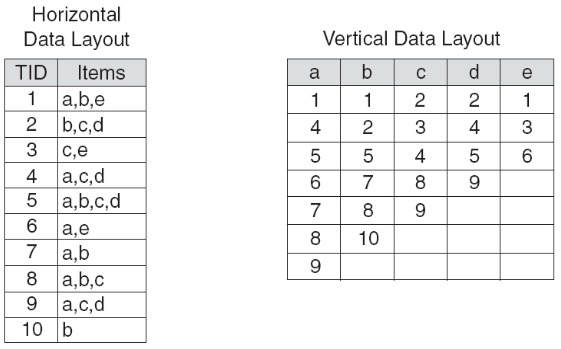
\includegraphics[scale=0.5]{pics/horizontal.png}
 				\caption{Horizontal and vertical data format}
 		\end{figure}

 	\clearpage
 	\section{FP-Growth Algorithm}

 		This section represents an alternative algorithm called {\bf FP-growth} that takes
 		a radically different approach to discovering frequent itemsets. This algorithm
 		encodes the data set using a compact data structure called an {\bf FP-tree} and
 		extracts frequent itemsets directly from this structure. 

 		{\bf FP-tree representation:} An FP-tree is a composed representation of the input data.
 		It is constructed by reading the data set one transaction at a time and mapping each
 		transaction onto the path in the FP-tree. As different transactions can have several items 
 		in common, their paths may overlap. 
 		Each node in the tree contains the label of an item along with a counter that shows
 		the number of transactions mapped onto the given path. 

 		\begin{enumerate}
 			\item The data set is scanned once to determine the support count of each item.
 			Infrequent items are discarded, while the frequent items  are sorted in decreasing
 			support count. For the data set in the figure, a is the most frequent item, 
 			followed by b, c, d and e.
 			\item The algorithm makes a second pass over the data to construct the tree.
 			After reading the first transaction, \{a,b\}, the nodes labeled as a and b are created.
 			A path is then formed from null $\rightarrow$ a $\rightarrow$ b to endcode
 			the transaction. Every node along the path has now a frequency count of 1.
 			\item The process of adding each transaction to a path and increasing the count along
 			the path continues until every transaction has been mapped onto one of the paths in the 
 			FP-tree. The final result is given in figure 6.19. 
 		\end{enumerate}
 		
 		\begin{figure}[H]
 				\centering
 				\includegraphics[scale=0.7]{pics/fptree.png}
 				\caption{Constructing of an FP-tree}
 		\end{figure}


 	\section{Evaluation of Association Patterns}


 		{\bf \Huge \color{red} PENSUM ???}
	\clearpage
	\chapter{Cluster Analysis: Basic Concepts and Algorithms}

{\bf Clustering for understanding:} classes, or conceptually meaningful groups of 
objects that share common characteristics, play an important role in how people 
analyze and describe the world. Indeed, human beings are skilled at dividing
objects into groups (clustering) and assigning particular objects to these 
groups (classification).

{\bf Clustering for utility:} In the context of utility, cluster analysis is the
study of techniques for finding the most representative cluster prototypes. 
Some of these techniques are: summarization, compression and finding nearest neighbors.

\clearpage
\section{Overview}
	
	\subsection{What Is Cluster Analysis}

	Cluster analysis groups data objects based only on information found in the 
	data that describes the objects and their relationships. The goal is that the
	objects within a group be similar (or related) to one another and different
	from (or unrelated to) to the objects in other groups. 

	Clustering can also be regarded as a form of classification.
	In contrast, classification in the sense of chapter 4 is {\bf supervised classifiction};
	i.e., new, unlabeled objects are assigned a class label using a model developed
	from objects with known class labels. For this reason, cluster analysis
	is sometimes referred to as {\bf unsupervised classification}.

	The terms {\bf segmentation} and {\bf partitioning} are somtimes used as
	synonyms for clustering.

	\subsection{Different Types of Clusterings}

		An entire collection of clusters is commonly referred to as {\bf clustering}, and
		in this section, we distinguish various types of clusterings: hierarchical (nested)
		vs. partitional (unnested), exclusive vs. overlapping vs. fuzzy, and complete vs. 
		partial. 

		\subsection*{Hierarchical vs. Partitional} 
		A {\bf partitional clustering} is simply a division of the set of data objects into
		non-overlapping subsets (clusters) such that each data object is in exactly one subset.
		If we permit clusters to have subclusters, then we obtain a {\bf hierarchical clustering},
		which is a set of nested clusters that are organized as a tree. Each node (cluster)
		in the tree (expect for the leaf nodes) is the union of its children (subclusters),
		and the root of the tree is the cluster containing all the objects. 

		\subsection*{Exclusive vs. Overlapping vs. Fuzzy}
		When a clustering is {\bf exclusive}, we assign each object to a single cluster.
		In the most general sense, an {\bf overlapping} or {\bf non-exclusive clustering} 
		is used to reflect the fact that an object can simultaneously belong to more than
		one group (class). For instance, a person at a university can be both an enrolled
		student and an employee of the university. 
		In {\bf Fuzzy clustering}, every object belongs to every cluster with a membership
		weight that is between 0 (absolutely doesn't belong) and 1 (absolutely belongs).
		In fuzzy clustering, we often impose the additional constraint that the sum of the
		weights for each object must equal to 1.  

		\subsection*{Complete vs. Partial}
		A {\bf complete clustering} assigns every object to a cluster, wheras a {\bf partial clustering}
		does not. The motivation for a partial clustering is that some objects in a data 
		set may not belong to well-defined groups. Many times objects in the data set may
		represent noise, outliners, or "uninteresting background."

	\clearpage
	\subsection{Different Types of Clusters}

		\begin{itemize}
			\item {\bf Well-seperated:} Figure 7.1a represents well-seperated clusters.
			Each point is closer to all of the points in its cluster than to any point 
			in another cluster.
			\item {\bf Prototype-Based:} Figure 7.1b shows a prototyped-based (center-based)
			clusters. Each point is closer to the center of its cluster than to the center of any
			other cluster. 
			\item {\bf Graph-Based:} If the data is represented as a graph, where the nodes
			are objects annd the links represent connections among objects, then a cluster can be
			defined as a {\bf connected component}; i.e., a group of objects that are connected
			to one another, but that have no connection to objects outside the group. An
			important example of graph-based clusters are {\bf contingency-based clusters}, where
			two objects are connected only if they are within a specified distance of each other. 
			Each point is closer to at least one point in its cluster than to any point in another 
			cluster, Figure 7.1c. 
			\item {\bf Density-Based:} A cluster is a dense region of objects that is surrounded by
			a region of low density. Figure 7.1d shows a density-based cluster.
			\item {\bf Shared-Property (Conceptual Clusters):} We can define a cluster as a set of 
			objects that share some property. Figure 7.1e shows an example of conceptual clusters.
		\end{itemize} 



		\begin{figure}[H]
			\centering
			\includegraphics[scale=0.6]{pics/clusters.png}
			\caption{Different types of clusters as illustrated by seys of two-dimensional points}
		\end{figure}

	\clearpage
	\section{K-means}
		This is a prototype-based, partitional clustering technique that attempts to find a
		user-specified number of clusters (K), which are represented by their centroids. 
		K-means defines a prototype in terms of a centroid, which is usually the mean of a 
		group of points. {\bf K-medoid} is almost the same as K-means with centroids, but a centroid
		does not to be an actual data point, while a mendoid does need to be an actual data point.

		{\bf The basic K-means algorithm:} we first choose K initial centroids, where K is a 
		user-specified parameter, namely, the number of clusters desired. Each data point is then
		assigned to the closest centroid, and each collection of ponts assigned to a centroid is a
		cluster. The centroid of each cluster is then updated based on the points assigned to the
		cluster. We repeat the assignment and update steps until no point changes cluster, or 
		equivalently, until the centroids remain the same.

		\begin{figure}[H]
			\centering
			\includegraphics[width=\textwidth]{pics/iterations.png}
			\caption{Using the k-means algorithm to find three clusters in sample data}

		\end{figure} 

		{\bf Assigning Points to the closest centroid:}	To assign a point to the closest centroid, 
		we need a proximity measure that quantifies the notion of "closest" for the specific data
		under consideration. Once we have a specified a proximity measure and an objective function, 
		the centroid that we should choose can often be determined mathematically. 

		{\bf Data in euclidean space:} Consider data whose proximity measure is Euclidean distance.
		For our objective function, which measures the quality of a clustering, we use the 
		{\bf sum of squared error (SSE)}, which is also known as scatter. In other words, we 
		calculate the error of each data point, i.e., its Euclidean distance to the closest centroid,
		and then compute the total sum of the squared errors. 

		\begin{equation}
			SSE = \sum_{i=1}^{K}\sum_{x E C_{i}}^{} dist(c_{i}, x)^{2}
		\end{equation}

		\begin{equation}
			c_{i} = \frac{1}{m_{i}} \sum_{x E C_{i}}^{} x
		\end{equation}

		\clearpage
		{\bf Document Data:} our objective is to maximize the similarity of the documents in a 
		cluster to the cluster centroid; this quantity is known as the {\bf cohesion} of the
		cluster. For this objective it can be shown that the cluster centroid is, as for
		Euclidean data, the mean. The analogous quantity to the total SSE is the total cohesion.

		\begin{equation}
			Total Cohesion = \sum_{i=1}^{K}\sum_{x E C_{i}}^{} cosine(x, c_{i})
		\end{equation}

		{\bf Choosing Initial Centroids:}\\
		\begin{itemize}
			\item Centroids are often choosen randomly
			\item Random otften gives a poor result because the probability of hitting a cluster.
			\item Possible solutions:
				\begin{itemize}
					\item Gjør klyngingen flere ganger og velg det beste (mht. SSE)
					(Sannsynligheten ikke på vår side!) 
					\item Sampling og bruk av hierarkisk klynging for å finne initielle 
					sentroider (Kun for lav verdi av K og små sample)
					\item Velg mer enn K punkt og velg blant disse • Feks. mest mulig separert
					(Gjort på sample for å redusere sjanse for outlier)
					\item Post/pre-prosessering 
					\item Bisecting K-means
				\end{itemize}
		\end{itemize}

		\begin{table}[H]
			\begin{tabular}{| l | l | p{8cm} |}
				\hline
				{\bf Proximity function} & {\bf Centroid} & {\bf Objective function} \\ \hline
				Manhattan ($L_{1}$) & median
				& Minimize sum of the $L_{1}$ distance of an object to its cluster centroid. \\ \hline
				Squared Euclidean ($L_{2}^{2}$) & mean
				& Minimize sum of the squared $L_{2}$ distance of an object to its cluster centroid \\ \hline
				cosine & mean 
				& Maximize sum of the cosine similarity of an object to its cluster centroid. \\ \hline
				Bergman Divergence & mean &
				Minimize sum of the Bergman divergence of an object to its cluster centroid. \\ \hline
			\end{tabular}
			\caption{Commom choices for proximity, centroids, and objective functions}
		\end{table}

		\subsection{K-means: Additional Issues}
			\begin{itemize}
				\item {\bf Handling empty clusters:}
				\item {\bf Outliners:}
				\item {\bf Reducing the SSE with postprocessing}
					\begin{itemize}
						\item Slit a cluster: The cluster with the largest SSE is usually chosen.
						\item Introduce a new cluster centroid: Often the point that is farthest from
						any cluster is chosen, of choose randomly. 
						\item Disperse a cluster: this as accomplished by removing the centroid that
						corresponds to the cluster and reassigning the points to other clusters. 
						Ideally, the cluster that is dispersed should be the one that increase the
						total SSE the least. 
						\item Merge two clusters: The clusters with the closests centroids are 
						typically chosen.
					\end{itemize}
				\item {\bf Updating centroids incrementally:} instead of updating cluster centroids
				after all points have been assigned to a cluster, the centroids can be updated
				incrementall, after each assignment of a point to a cluster. 
			\end{itemize}

		\subsection{Bisecting K-means}

		The bisecting K-means algorithm is a straightforward extension of the basic K-menas algorithm
		that is based on a simple idea: to obtain K clusters, split the set of all points into two
		clusters, select one of these clusters to split, and so on, until K clusters have been 
		produced. 

		\subsection{K-means and Different types of Clusters}

		K-means and its variations have a number of limitations with respect to finding different 
		types of clusters. In particular, K-means have difficulty detecting the "natural" clusters,
		when clusters have different size, different density or non-globular clusters. 

		
	\section{Agglomerative Hierarchical Clustering}
		{\bf Different types of hierarchical clustering:}
		\begin{itemize}
			\item {\bf Agglomerative:} start at the points as individual clusters
			and, at each step, merge the closest pair of clusters.
			\item {\bf Divisive:} Start with one, all-inclusive cluster, and at each
			step, split a cluster until only singelton clusters of individual points
			remain. 
		\end{itemize}

		A hierarchical clustering is often displayed graphically using a tree-like diagram
		called a {\bf dendrogram}, which displays both the cluster-subcluster relationship
		and the order in which the clusters are merged (agglomerative view) or split 
		(divisive view). 

		\begin{figure}[H]
			\centering
			\includegraphics[scale=0.3]{pics/hierarchical.png}
			\caption{Dendrogram and nested cluster diagram}
		\end{figure}

		\clearpage
		{\bf Defining Proximity between Clusters}
		\begin{itemize}
			\item {\bf MIN/single link:} defines cluster proximity as the proximity between the closest
			two points that are in different clusters, or using graph terms, the shortest edge between
			two nodes in different subsets of nodes. 
			\item {\bf MAX/CLIQUE/complete link:} takes the proximity between the farthest two points in different
			clusters to be the cluster proxximity, or using graph terms, the longest edge between 
			two nodes in different subsets of nodes. 
			\item {\bf Group average:} defines cluster proximity to be the average pairwise proximities
			(average length of edges) of all pairs of points from different clusters. 
		\end{itemize}

		\begin{figure}[H]
			\centering
			\includegraphics[width=\textwidth]{pics/minmax.png}
			\caption{Min, Max and group average}
		\end{figure}

		\clearpage
		\subsection{Specific Techniques}

		In this section we will go through an example of single and complete link with 
		data points. In the figure below, we see the example data of six points with x and y 
		positions and the distance from each point to all other points. We always start with 
		getting two clusters with 2 points in each that have the smallest distance, then 
		we start merging with MIN or MAX linking.
			
			\begin{figure}[H]
				\centering
				\includegraphics[scale=0.28]{pics/datapoints.png}
			\end{figure}

		{\bf Single Link (MIN):} for the single link or MIN version of hierarchical clustering, 
		the proximity of two clusters is defined as a minimum of the distance (maximum of the 
		similarity) between any points in the two different clusters. Using graph terminology, 
		if you start with all points as singleton clusters and add link between points one at 
		a time, shortest links first, then these single links combine the points into clusters. 
		The figure below shows the result of applying the single link technique to our example
		data set of six points.

		We see that the distance between point 3 and 6 is 0.11, and that is the height at which they
		are joined into one clusterin the dendrogram. As another example, the distance between
		clusters \{3,6\} and \{2,5\} is given by:

		{\color{red} $dist(\{3,6\}, \{2,5\})$ = min(dist(3,2), dist(6.2), dist(3,5), dist(6,5))
		= min(0.15, 0.25, 0.28, 0.39) = 0.15}


			\begin{figure}[H]
				\centering
				\includegraphics[scale=0.3]{pics/minlink.png}
				\caption{Results from the single link}
			\end{figure}			
		\clearpage
		{\bf Complete Link (MAX/CLIQUE):} For the complete link version of the  hierarchical clustering,
		the proximity of two clusters is defined as the maximum of the distance  (minimum of the 
		similarity) between any two points in the two different clusters. Using graph terminology,
		if you start with all points as singleton clusters and add links between points one at a time,
		shortests links first, then a group of points is not a cluster until all points in it are 
		completely linked, i.e., form a clique. 
		\{3,6\} and \{5,2\} is the two first clusters. We know need to merge with a new point or cluster:

		{\color{red} dist(\{3,6\}, \{4\}) = max(dist(3,4), dist(6,4)) = max(0.15, 0.22) = 0.22}

		{\color{blue} dist(\{3,6\}, \{2,5\}) = max(dist(3,2), dist(6,2), dist(3,5), dist(6,5)) = 
		max(0.15, 0.25, 0.28, 0.39)	= 0.39}

		{\color{orange} dist(\{3,6\}, \{1\}) = max(dist(3,1), dist(6,1)) = max(0.22, 0.23) = 0.23}

		We can see that merging cluster \{3, 6\} with \{4\} gives the minimum distance. It is
		very confusing using both terms min and max!

			\begin{figure}[H]
				\centering
				\includegraphics[scale=0.3]{pics/completelink.png}
				\caption{Results from the complete link}
			\end{figure}

		\clearpage
		{\bf Group Average:} For the group average version of hierarchical clustering, the
		proximity of two clusters is defined as the average pairwise proximity among all pairs of
		points in the different clusters. This is an intermediate approach between the single
		and complete link appraches. Thus, for group average, the cluster proximity 
		$proximity(C_{i}, C_{j})$ of clusters $C_{i}$ and $C_{j}$, which are of size $m_{i}$
		and $m_{j}$, respectively, is expressed by the following equation:

		\begin{equation}
			proximity(C_{i}, C_{j}) = \frac{\sum_{x \in C_{j}, y \in C_{j}} proximity(x,y)}{m_{i}*m_{j}}
		\end{equation}

		Here are some calculations from the 4'th iteration:

		{\color{red} dist(\{3, 6, 4\}, \{1\}) = (0.22 + 0.37 + 0.23) / (3*1) = 0.28}

		{\color{blue} dist(\{2, 5\}, \{1\}) = (0.2357 + 0.3421) / (2*1) = 0.2889}

		{\color{orange} dist(\{3, 6, 4\}, \{2, 5\}) = (0.15, 0.28, 0.25, 0.39, 0.2, 0.29) / (3*2) = 0.26}

		Here we choose to merge cluster \{3,6,4\} with cluster \{2,5\} because of the lowest
		proximity value. 


			\begin{figure}[H]
				\centering
				\includegraphics[scale=0.3]{pics/average.png}
				\caption{Results from the group average}
			\end{figure}

		{\bf Ward's method:} the proximity between two clusters is defined as the increase in 
		the squared error that results when two clusters are merged. This method uses the same
		objective function as k-means clustering. 
			
			\begin{figure}[H]
				\centering
				\includegraphics[scale=0.3]{pics/ward.png}
				\caption{Results from the Ward's method}
			\end{figure}
		\clearpage
		{\bf Strengths and weaknesses with hiaarchical clustering methods:}
			\begin{itemize}
				\item Single link (MIN)
					\begin{itemize}
						\item Fordel: Kan håndtere ikkeelliptiske former 
						\item Svakhet: Sensitiv til støy og outliers 
					\end{itemize}
				\item Complete link (MAX)
					\begin{itemize}
						\item Fordel: Mindre følsom for støy og outliers 
						\item Svakheter: Gir ofte oppdeling av store klynger,
						Tilbøyelighet mot kuleformet klynger, sensitiv til støy og outliers.
					\end{itemize}
				\item Group Average:
					\begin{itemize}
						\item Kompromiss mellom MIN og MAX 
						\item Styrke: Mindre følsom for støy og outliers 
						\item Svakhet: Tilbøyelighet mot kuleformet klynger
						\item Problem: dyrt å utregne
					\end{itemize}
			\end{itemize}

	\section{DBSCAN}		

		Density-based clustering locates regions of high density that are seperated
		from one another by regions of low density. DBSCAN is a simple and effective
		density-based clustering algorithm. 

		\subsection{Traditional Density: Center-Based Approach}

		{\bf Classification of points according to center-based density:}
		\begin{itemize}
			\item {\bf Core points:} in the enterior of a dense region (a core point).
			A point is a core point if the number of points within a given neigborhood around the 
			point as determined by the distance function and a user specified distance 
			parameter, {\it Eps}, exceeds a certain threshold, {\it MinPts}, which is also a
			user-specified parameter.  
			\item {\bf Border points:} on the edge of a dense region (a border point).
			\item {\bf Noise points:} in a sparsely occupied region (a noise or background point).
		\end{itemize}


			\begin{figure}[H]
				\centering
				\includegraphics[width=\textwidth]{pics/dbscan.png}
			\end{figure}

		\subsection{DBSCAN Algorithm}

			The DBSCAN can be informally described as follows. Any two core points
			that are close enough - within a distance {\it Eps} of ine another - 
			are put in the same cluster. Likewise, any border point that is close 
			enough to a core point is put in the same cluster as the core point.
			(Ties may need to be resolved if a border point is close to core points
			from different clusters.) Noise points are discarded. 

			\begin{enumerate}
				\item Label all points as core, border, or noise points.
				\item Eliminate noise points
				\item Put an edge between all core points that are within {\it Eps} of each other
				\item Make each group of connected core points into a separate cluster
				\item Assign each border point to one of the clusters of its associated core points.
			\end{enumerate}

			\begin{figure}[H]
				\centering
				\includegraphics[scale=0.5]{pics/dbscan2.png}
				\caption{1) Original data points, 2) {\color{green}core points}, {\color{blue}border points}, and
				{\color{red}noise points}.}
			\end{figure}

			{\bf Strengths and Weaknesses}
				\begin{itemize}
					\item {\bf Fungerer når:} Motstandsdyktig mot støy og kan håndtere klynger med forskjellige former 
					og størrelse
					\item {\bf Fungerer ikke når:} Varierende tetthet, Høydimensjonale data.
					\item Er sensitiv i forhold til valg av eps og MinPts.
					\item Cluster som ligger inne i støy fungerer ikke så bra. 
				\end{itemize}

	\clearpage
	\section{Cluster Evaluation}

		In supervised classification, the evaluation of the resulting classification model
		is an integral part of the proces of developing a classification model, and
		there are well-accepted evaluation measures and procedures, e.g., accuracy
		and cross-validation, respectively. However, because of its very nature, cluster
		evaluation is not a well-developed or commonly used part of cluster analysis.

		There are a number of different clusters - in some sense, each clustering 
		algorithm defines its own type of clusters - it may seem that each situation 
		might require a different evaluation measure. Here are a clustering example with
		different algorithms used:

		\begin{figure}[H]
			\centering
			\includegraphics[scale=0.4]{pics/threeclusters.png}
		\end{figure}

		{\bf Important issues for cluster validation:}
		\begin{enumerate}
			\item Determining the cluster tendency of a set of data, i.e., distinguishing
			between wheter non-random structure actually exists in the data.
			\item Determining the correct number of clusters
			\item Evaluating how well the results of a cluster analysis fit the data
			without reference to external information.
			\item Comparing the results of a cluster analysis to externally known results,
			such as externally provided class labels.
			\item Comparing two sets of clusters to determine which is better. 
		\end{enumerate}

		\clearpage
		Evaluation measures, or indices, that are applied to judge various aspects of cluster validity
		are traditionally classified into the following three types:

			\begin{itemize}
				\item {\bf Unsupervised:} measure the goodness of a clustering structure without
				respect to external information. An example of this is SSE. 
				Unsupervised measures of cluster validity are often further divided into
				two classes: measures of {\bf cluster cohesion} (compactness, tightness), which
				determine how closely related the objects in a cluster are, and measures
				of {\bf cluster separation} (isolation), which determine how distinct or well
				separated a cluster is from other clusters. Unsupervised measures are often
				called {\bf internal indices} because they use only information present in the
				data set.
				\item {\bf Supervised:} measures the extent to which the clustering structure
				discovered by a clustering algorithm matches some external structure. 
				An example of supervised index is entropy, which measures how well a cluster
				labels match externally supplied class labels. Supervised measures are 
				often called {\bf external indices} becuase they use information not present
				in the data set. 
				\item {\bf Relative:} Compares different clustering or clusters. A relative 
				cluster evaluation measure is supervised or unsupervised evaluation measure 
				that is used for the purpose of comparison. As an example, two K-means clusterings
				can be compared using either the SSE or entropy. 
			\end{itemize}

		\subsection{Unsupervised Cluster Evaluation Using Cohesion and Sparation}
			In general, we can consider expressing overall cluster validity for a set of 
			K clusters as a weighted sum of the validity of individually clusters:

				\begin{equation}
					overall Validity = \sum_{i=1}^{K} w_{i} validity(C_{i})
				\end{equation}

			The validity function can be cohesion, spearation, or some combination of 
			these quantities.

			{\bf Graph-based view of Cohesion and separation}

			For graph-based clusters, the cohesion of a cluster can be defined as the sum
			of the weights of the links in the proximity graph that connect points whitin 
			the cluster. 
			Likewise, the separation between two clusters can be measured by the sum of
			weights of the links from points in one cluster to point in the other cluster.
			The proximity function can be a similarity, a dissimilarity, or a simple function
			of these quantities. 

				\begin{equation}
					cohesion(C_{i}) = \sum_{x \in C_{i}, y \in C_{i}} proximity(x,y)
				\end{equation} 

				\begin{equation}
					separation(C_{i}, C_{j}) = \sum_{x \in C_{i}, y \in C_{j}} proximity(x,y)
				\end{equation} 

			\begin{figure}[H]
				\centering
				\includegraphics[scale=0.3]{pics/graphbased.png}
			\end{figure}


			{\bf Prototype-based View of Cohesion and Separation}

			For prototype-based clusters, the cohesion of a cluster can be defined as the sum
			of proximties with respect to the prototype (centroid or mendoid) of the cluster.

			\begin{equation}
				cohesion(C_{i}) = \sum_{x \in C_{i}} proximity(x, c_{i})
			\end{equation}

			\begin{equation}
				separation(C_{i}, C_{j}) = proximity(c_{i}, c_{j})
			\end{equation}

			\begin{equation}
				separation(C_{i}) = proximity(c_{i}, c)
			\end{equation}

			$c_{i}$ is the prototype (centroid) of cluster $C_{i}$, and c is the overall
			prototype (centroid). 

			\begin{figure}[H]
				\centering
				\includegraphics[scale=0.3]{pics/prototypebased.png}
			\end{figure}

			{\bf Evaluating Individual Clusters and Objects}

				So far, we have focused on using cohesion and separation in the overall
				evaluation of a group of clusters. Many of these measures of cluster
				validity also can be used to evaluate individual clusters and objects.

				A cluster that has a high value of cohesion may be considered better than
				a cluster that has a lower value. This information often can be used to 
				improve the quality of a clustering. If for example, a cluster is not
				very cohesive, then we may want to split it into serveral subclusters. 
				On the other hand, if two clusters are relatively cohesive, ut not
				well separated, we may want to merge them into a single cluster. 

				We can also evaluate the objects within a cluster in terms of their
				contribution to the overall cohesion or separation of the cluster. 
				Objects that contribute more to the cohesion and separation are near the 
				"interior" of the cluster. Those objects for which the opposite is true
				are probably near the "edge" of the cluster. 

				{\bf The Silhouette Coefficient:}

				The popular method of silhouette coefficients combines both cohesion and
				separation. The following steps explain how to compute the silhouette coefficient
				for an individual point., a process that consists of the following three steps.
				We use distances, but an analogous approach can be used for similarities.

				\begin{enumerate}
					\item For the $i^{th}$ object, calculate its average distance to all other
					objects in its cluster. Call this value $a_{i}$.
					\item For the $i^{th}$ object annd any cluster not containing the object,
					calculate the object's average distance to all the objects in the given
					cluster. Find the minimum such value with respect to all clusters; call
					this value $b_{i}$.
					\item For the $i^{th}$ object, the silhouette coefficient is 
					$s_{i} = (b_{i} - a_{i})/max(a_{i},b_{i})$.
				\end{enumerate}

				The value of the silhouette can vary between -1 and 1. A negative value is
				undesirable because this corresponds to a case in which $a_{i}$, the average
				distance to points in the cluster, is greater than $b_{i}$, the minimum
				average distance to points in another cluster. We want the silhouette
				coefficient to be positive, and for $a_{i}$ to be as close to 0 as possible,
				since the coefficient assumes its maximum value of 1 when $a_{i}$ = 0.

				We can compute the average silhouette coefficient of a cluster by simply
				taking the average of the shilouette coefficients of points belonging to the
				cluster. An overall measure of the goodness of a clustering can be obtained
				by computing the average silhouette coefficient of all points. 


		\subsection{Unsupervised Cluster Evaluation Using the Proximity Matrix}

			In this section, we examine a couple of unsupervised approaches for assessing
			cluster validity that are based on the proximity matrix. 

			{\bf Measuring Cluster Vality via Correlation}

			If we are given the similarity matrix for a data set and the cluster labels from
			a cluster analysis of the data set, then we can evaluate the goodness of the 
			clustering by looking at the correlation between {\bf actual similarity matrix} and an 
			{\bf ideal version of the similarity matrix} based on the cluster labels. 

			More Specifically, an ideal cluster is one whose points have a similarity
			of 1 to all points in the cluster, and a similarity of 0 to all points
			in other clusters.

			The {\bf ideal similarity matrix} is constructed by creating a matrix that has one
			row and one column  for each data point, and assigning a 1 to an entry if the 
			associated pair of points belongs to the same cluster. All other entries are 0.
			High correlation between the ideal and actual simularity matrices indicates
			that the points that belong to the same cluster are close to each other, while
			low correlation indicates the opposite. 
			Since the actual and ideal similarity matrices are symmetric, the correlation is
			calculated only among the n(n-1)/2 entries below or above the diagonal of the matrices.


		\subsection{Internal goals: Cohesion and seperation}

			\begin{figure}[H]
				\centering
				\includegraphics[scale=0.5]{pics/cosep.png}
			\end{figure}
			\begin{figure}[H]
				\centering
				\includegraphics[scale=0.5]{pics/cosep2.png}
			\end{figure}

		\subsection{Internal goals: ENtropy and Purity}

		\begin{figure}[H]
				\centering
				\includegraphics[scale=0.5]{pics/entpu.png}
			\end{figure}



\end{document}



